%%%%%%%%%%%%%%%%%%%%%%%%%%%%%%%%%%%%%%%%%
% Masters/Doctoral Thesis 
% LaTeX Template
% Version 1.43 (17/5/14)
%
% This template has been downloaded from:
% http://www.LaTeXTemplates.com
%
% Original authors:
% Steven Gunn 
% http://users.ecs.soton.ac.uk/srg/softwaretools/document/templates/
% and
% Sunil Patel
% http://www.sunilpatel.co.uk/thesis-template/
%
% License:
% CC BY-NC-SA 3.0 (http://creativecommons.org/licenses/by-nc-sa/3.0/)
%
% Note:
% Make sure to edit document variables in the Thesis.cls file
%
%%%%%%%%%%%%%%%%%%%%%%%%%%%%%%%%%%%%%%%%%

%----------------------------------------------------------------------------------------
%	PACKAGES AND OTHER DOCUMENT CONFIGURATIONS
%----------------------------------------------------------------------------------------

\documentclass[11pt, oneside]{Thesis} % The default font size and one-sided printing (no margin offsets)

\graphicspath{{Pictures/}} % Specifies the directory where pictures are stored
\usepackage[parfill]{parskip}
\usepackage{graphicx}				% Use pdf, png, jpg, or eps§ with pdflatex; use eps in DVI mode
\usepackage{subfig}
								% TeX will automatically convert eps --> pdf in pdflatex
\usepackage{amssymb}
\usepackage{amsmath}
\usepackage{natbib}

\usepackage[TS1,T1]{fontenc}
%\usepackage{fourier, heuristica}
\usepackage{array, booktabs}
\usepackage[x11names]{xcolor}
\usepackage{colortbl}
\usepackage{caption}
\usepackage{bbm}
\usepackage{amssymb}
\usepackage{amsmath}
\usepackage{mathtools}
\usepackage{float}
\usepackage[]{algorithm2e}
\DeclareCaptionFont{blue}{\color{LightSteelBlue3}}
\DeclareMathOperator*{\argmax}{\arg\!\max}

% \newcommand{\foo}{\color{LightSteelBlue3}\makebox[0pt]{\textbullet}\hskip-0.5pt\vrule width 1pt
% \hspace{\labelsep}}

\newcommand{\p}{\text{p}}

% \usepackage[square, numbers, comma, sort&compress]{natbib} % Use the natbib reference package - read up on this to edit the reference style; if you want text (e.g. Smith et al., 2012) for the in-text references (instead of numbers), remove 'numbers' 
\hypersetup{urlcolor=blue, colorlinks=true} % Colors hyperlinks in blue - change to black if annoying
\title{\ttitle} % Defines the thesis title - don't touch this

\begin{document}

\frontmatter % Use roman page numbering style (i, ii, iii, iv...) for the pre-content pages

\setstretch{1.3} % Line spacing of 1.3

% Define the page headers using the FancyHdr package and set up for one-sided printing
\fancyhead{} % Clears all page headers and footers
\rhead{\thepage} % Sets the right side header to show the page number
\lhead{} % Clears the left side page header

\pagestyle{fancy} % Finally, use the "fancy" page style to implement the FancyHdr headers

\newcommand{\HRule}{\rule{\linewidth}{0.5mm}} % New command to make the lines in the title page

% PDF meta-data
\hypersetup{pdftitle={\ttitle}}
\hypersetup{pdfsubject=\subjectname}
\hypersetup{pdfauthor=\authornames}
\hypersetup{pdfkeywords=\keywordnames}

%----------------------------------------------------------------------------------------
%	TITLE PAGE
%----------------------------------------------------------------------------------------

\begin{titlepage}
\begin{center}

\textsc{\LARGE \univname}\\[1.5cm] % University name
\textsc{\Large Master Thesis}\\[0.5cm] % Thesis type

\HRule \\[0.4cm] % Horizontal line
{\huge \bfseries \ttitle}\\[0.4cm] % Thesis title
\HRule \\[1.5cm] % Horizontal line
 
\begin{minipage}{0.4\textwidth}
\begin{flushleft} \large
\emph{Author:}\\
{\authornames} % Author name - remove the \href bracket to remove the link
\end{flushleft}
\end{minipage}
\begin{minipage}{0.4\textwidth}
\begin{flushright} \large
\emph{Supervisor:} \\
{\supname} % Supervisor name - remove the \href bracket to remove the link  
\end{flushright}
\end{minipage}\\[3cm]
 
\large \textit{A thesis submitted in fulfilment of the requirements\\ for the degree of \degreename}\\[0.3cm] % University requirement text
\textit{in the}\\[0.4cm]
\groupname\\\deptname\\[2cm] % Research group name and department name
 
{\large \today}\\[4cm] % Date
%\includegraphics{Logo} % University/department logo - uncomment to place it
 
\vfill
\end{center}

\end{titlepage}

%----------------------------------------------------------------------------------------
%	DECLARATION PAGE
%	Your institution may give you a different text to place here
%----------------------------------------------------------------------------------------

\Declaration{

\addtocontents{toc}{\vspace{1em}} % Add a gap in the Contents, for aesthetics

I, \authornames, declare that this thesis titled, '\ttitle' and the work presented in it are my own. I confirm that:

\begin{itemize} 
\item[\tiny{$\blacksquare$}] This work was done wholly or mainly while in candidature for a research degree at this University.
\item[\tiny{$\blacksquare$}] Where any part of this thesis has previously been submitted for a degree or any other qualification at this University or any other institution, this has been clearly stated.
\item[\tiny{$\blacksquare$}] Where I have consulted the published work of others, this is always clearly attributed.
\item[\tiny{$\blacksquare$}] Where I have quoted from the work of others, the source is always given. With the exception of such quotations, this thesis is entirely my own work.
\item[\tiny{$\blacksquare$}] I have acknowledged all main sources of help.
\item[\tiny{$\blacksquare$}] Where the thesis is based on work done by myself jointly with others, I have made clear exactly what was done by others and what I have contributed myself.\\
\end{itemize}
 
Signed:\\
\rule[1em]{25em}{0.5pt} % This prints a line for the signature
 
Date:\\
\rule[1em]{25em}{0.5pt} % This prints a line to write the date
}

\clearpage % Start a new page

%----------------------------------------------------------------------------------------
%	QUOTATION PAGE
%----------------------------------------------------------------------------------------

% \pagestyle{empty} % No headers or footers for the following pages

% \null\vfill % Add some space to move the quote down the page a bit

% \textit{``Thanks to my solid academic training, today I can write hundreds of words on virtually any topic without possessing a shred of information, which is how I got a good job in journalism."}

% \begin{flushright}
% Dave Barry
% \end{flushright}

% \vfill\vfill\vfill\vfill\vfill\vfill\null % Add some space at the bottom to position the quote just right

% \clearpage % Start a new page

%----------------------------------------------------------------------------------------
%	ABSTRACT PAGE
%----------------------------------------------------------------------------------------

\addtotoc{Abstract} % Add the "Abstract" page entry to the Contents

\abstract{\addtocontents{toc}{\vspace{1em}} % Add a gap in the Contents, for aesthetics

The Thesis Abstract is written here (and usually kept to just this page). The page is kept centered vertically so can expand into the blank space above the title too\ldots
}

\clearpage % Start a new page

%----------------------------------------------------------------------------------------
%	ACKNOWLEDGEMENTS
%----------------------------------------------------------------------------------------

\setstretch{1.3} % Reset the line-spacing to 1.3 for body text (if it has changed)

\acknowledgements{\addtocontents{toc}{\vspace{1em}} % Add a gap in the Contents, for aesthetics

The acknowledgements and the people to thank go here, don't forget to include your project advisor\ldots
}
\clearpage % Start a new page

%----------------------------------------------------------------------------------------
%	LIST OF CONTENTS/FIGURES/TABLES PAGES
%----------------------------------------------------------------------------------------

\pagestyle{fancy} % The page style headers have been "empty" all this time, now use the "fancy" headers as defined before to bring them back

\lhead{\emph{Contents}} % Set the left side page header to "Contents"
\tableofcontents % Write out the Table of Contents

\lhead{\emph{List of Figures}} % Set the left side page header to "List of Figures"
\listoffigures % Write out the List of Figures

\lhead{\emph{List of Tables}} % Set the left side page header to "List of Tables"
\listoftables % Write out the List of Tables

%----------------------------------------------------------------------------------------
%	ABBREVIATIONS
%----------------------------------------------------------------------------------------

% \clearpage % Start a new page

% \setstretch{1.5} % Set the line spacing to 1.5, this makes the following tables easier to read

% \lhead{\emph{Abbreviations}} % Set the left side page header to "Abbreviations"
% \listofsymbols{ll} % Include a list of Abbreviations (a table of two columns)
% {
% \textbf{LAH} & \textbf{L}ist \textbf{A}bbreviations \textbf{H}ere \\
% %\textbf{Acronym} & \textbf{W}hat (it) \textbf{S}tands \textbf{F}or \\
% }

%----------------------------------------------------------------------------------------
%	PHYSICAL CONSTANTS/OTHER DEFINITIONS
%----------------------------------------------------------------------------------------

% \clearpage % Start a new page

% \lhead{\emph{Physical Constants}} % Set the left side page header to "Physical Constants"

% \listofconstants{lrcl} % Include a list of Physical Constants (a four column table)
% {
% Speed of Light & $c$ & $=$ & $2.997\ 924\ 58\times10^{8}\ \mbox{ms}^{-\mbox{s}}$ (exact)\\
% % Constant Name & Symbol & = & Constant Value (with units) \\
% }

%----------------------------------------------------------------------------------------
%	SYMBOLS
%----------------------------------------------------------------------------------------

% \clearpage % Start a new page

% \lhead{\emph{Symbols}} % Set the left side page header to "Symbols"

% \listofnomenclature{lll} % Include a list of Symbols (a three column table)
% {
% $a$ & distance & m \\
% $P$ & power & W (Js$^{-1}$) \\
% % Symbol & Name & Unit \\

% & & \\ % Gap to separate the Roman symbols from the Greek

% $\omega$ & angular frequency & rads$^{-1}$ \\
% % Symbol & Name & Unit \\
% }

%----------------------------------------------------------------------------------------
%	DEDICATION
%----------------------------------------------------------------------------------------

% \setstretch{1.3} % Return the line spacing back to 1.3

% \pagestyle{empty} % Page style needs to be empty for this page

% \dedicatory{For/Dedicated to/To my\ldots} % Dedication text

% \addtocontents{toc}{\vspace{2em}} % Add a gap in the Contents, for aesthetics

%----------------------------------------------------------------------------------------
%	THESIS CONTENT - CHAPTERS
%----------------------------------------------------------------------------------------

\mainmatter % Begin numeric (1,2,3...) page numbering

\pagestyle{fancy} % Return the page headers back to the "fancy" style

% Include the chapters of the thesis as separate files from the Chapters folder
% Uncomment the lines as you write the chapters

% Chapter 1

\chapter{Introduction} % Main chapter title

\label{Chapter1} % For referencing the chapter elsewhere, use \ref{Chapter1} 

\lhead{Chapter 1. \emph{Introduction}} % This is for the header on each page - perhaps a shortened title

%----------------------------------------------------------------------------------------

\section{Motivation}

CERN (Centre Europ\'een de la Recherche Nucl\'eaire) is the foremost European particle physics research laboratory, located on the border of France and Switzerland to the west of Geneva. The organisation, employing as many as 15,000 staff, fellows, and students at a time, is the global leader in high energy physics research, centered around massive particle collision experiments in the Franco-Swiss subterrain. INSPIRE-HEP (inspirehep.net) is an online open access digital library for high energy physics (HEP) papers built by an international collaboration of particle physics laboratories. INSPIRE-HEP derives from the older SPIRES project (\cite{gentil2009information}), and mounted upon the Invenio digital library software package. The digital library comprises of over one million HEP articles, theses and books, each painstakingly curated by professional librarians. As in most domains, such manual work may be enhanced with the assistance of automated processes, such as software systems based on state-of-the-art computer science techniques. Of particular interest is the annotation of scientific articles, that is, extracting a document's metadata from its \emph{content} such that it may be represented as an identifiable entity of the digital library. We refer to this as the problem of \emph{automatic metadata extraction} (AME). Though such technology is mainstream, at present INSPIRE-HEP has only limited solutions to this problem, relying heavily on tedious curation to complete the work. The problem of AME (Chapter \ref{Chapter3}) has been described as one of the hardest in document engineering \cite{souza2014arctic}, and a range of approaches to solving the problem exist, the most successful of which are machine learning techniques. This thesis presents a state-of-the-art open-source software for metadata extraction, GROBID, a system based on machine learning approaches, and shows how HEP papers have particular characteristics that require specialised extensions and feature engineering to improve the accuracy of extraction. Of particular note is the way a HEP paper may contain collaborations of thousands of authors (refer to Chapter \ref{Chapter4}). This alters the document layout drastically, creating structures unseen by baseline models. The requirements are therefore twofold:

\begin{enumerate}
\item to train models on a custom HEP training set, and;
\item to engineer specialised features conducive to better generalisation on HEP papers.
\end{enumerate}

\section{Aims}

Above all, we hypothesise the HEP use case: a qualitative difference in both the content and layout of a HEP article compared with other scientific articles, moreover implying the value of specialised model training and feature engineering. These differences are in fact directly observable in any representative HEP corpus, as we see in Chapter \ref{Chapter4}. The availability of a baseline dataset, in addition to our own custom HEP dataset, allow us to further experiment with hybrid datasets. This thesis proposes a set of features for models within the GROBID cascade (see Chapter \ref{Chapter3}). In short, our aims are:

\begin{enumerate}
\item to demonstrate the qualitative difference between HEP and general papers;
\item to propose improvements to model features, with suitable justifications;
\item to run experiments to confirm or reject our improvements, and;
\item to draw conclusions about what characterises good feature engineering.
\end{enumerate}

\section{Main Results}

The results of our 66 cross-validated experiments are presented in Chapter \ref{Chapter5}. These results confirm our initial hypothesis about HEP papers, as well as many of our intuitions. Concretely, we found improvements for each of the two GROBID models that we addressed, namely the \emph{header} model for processing article front matter, as well as the \emph{segmentation} model, the most important model in the cascade. In each case we found two feature variations to make substantial improvements over the baseline evaluations, making error reductions as great as $20\%-25\%$ for the most important classes.

\section{Outline}

In Chapter \ref{Chapter2} we provide a discussion of the relevant machine learning techniques, along with their solution algorithms, up to and including the state-of-the-art conditional random fields (CRF). In Chapter \ref{Chapter3} we present the problem of automatic metadata extraction, and the leading open-source software for the task, GROBID. Then, in Chapter \ref{Chapter4}, we showcase our propositions for improvements and extensions to the baseline models. In Chapter \ref{Chapter5} we present the results of our work and finally in Chapter \ref{Chapter6} we conceive of ways our research may be continued and extended.
% Chapter Template

\chapter{Supervised Sequence Learning} % Main chapter title

\label{Chapter2} % Change X to a consecutive number; for referencing this chapter elsewhere, use \ref{ChapterX}

\lhead{Chapter 2. \emph{Supervised Sequence Learning}} % Change X to a consecutive number; this is for the header on each page - perhaps a shortened title

%----------------------------------------------------------------------------------------
%	SECTION 1
%----------------------------------------------------------------------------------------

\emph{In this chapter we present the state-of-the-art technique for metadata extraction, conditional random fields (CRF). For completeness, we include a background history of related machine learning techniques and their associated optimisation algorithms. We begin with a presentation of Hidden Markov Models (HMM) and their inference algorithms. Following this we present multinomial logistic regression. From these former topics we show how their ideas are combined to produce Maximum Entropy Markov Models (MEMM) and CRFs. Notably, we pinpoint the part of the mathematical model relevant to our work on feature engineering. Finally, we describe Wapiti, a general-purpose software engine for training and tagging with CRF models.}

\section{Hidden Markov Models}

Hidden Markov models (HMMs) are a staple of natural language processing (NLP) and other engineering fields. A HMM models a probability distribution over an unknown, \emph{hidden} sequence of state variables of length $T$, $\mathbf{y} = (y_1, y_2, ..., y_T)$, whose elements take on values in a finite set of states, $S$, and follow a Markov process. For each element in this hidden sequence, there is a corresponding observation element, forming a sequence of \emph{observations}, $\mathbf{x} = (x_1, x_2, ..., x_T)$, similarly taking values in a finite set, $O$. The graphical structure of a HMM (Figure \ref{fig:HMM}) shows the dependencies between consecutive hidden states (these are modelled with \emph{transition} probabilities), and states and their observations (modelled with \emph{emission} probabilities). The first dependency is referred to as the Markov condition, which postulates the dependency of each hidden state, $y_t$, on its k precursors in the hidden sequence, namely, $\mathbf{y}_{t-k:t-1}$\footnote{In the following we use the notation $\mathbf{x}_{a:b}$ to refer to the elements of vector $\mathbf{x}$ from index $a$ through $b$ inclusive.}. In the discussion that follows, we assume the Markov condition to be of first degree, that is, $k =1$. Incidentally, higher-order HMMs may always be reconstructed to this simplest form (\cite{reference}). The second dependency may be referred to as \emph{limited lexical conditioning}, referring to the dependency of an observation only on its hidden state. Properties of the model may then be deduced through statistical inference, for example, a prediction of the most likely hidden sequence can be computed with the Viterbi algorithm (Section \ref{sec:viterbi}).

HMMs have been shown to be successful in statistical modelling problems. In Part of Speech (PoS) tagging, a classic NLP problem for disambiguating natural language sentences, the parts of speech (nouns, verbs, and so on) of a word sequence (sentence) are modelled as hidden states, and the words themselves are the observations. The PoS sequence may be modelled and predicted for as a HMM. Even a simple HMM can achieve an accuracy of well over $90\%$. The problem of metadata extraction is clearly similar in form to PoS tagging, as we further show in Chapter \ref{Chapter3}.

\begin{figure}[!ht]
\center
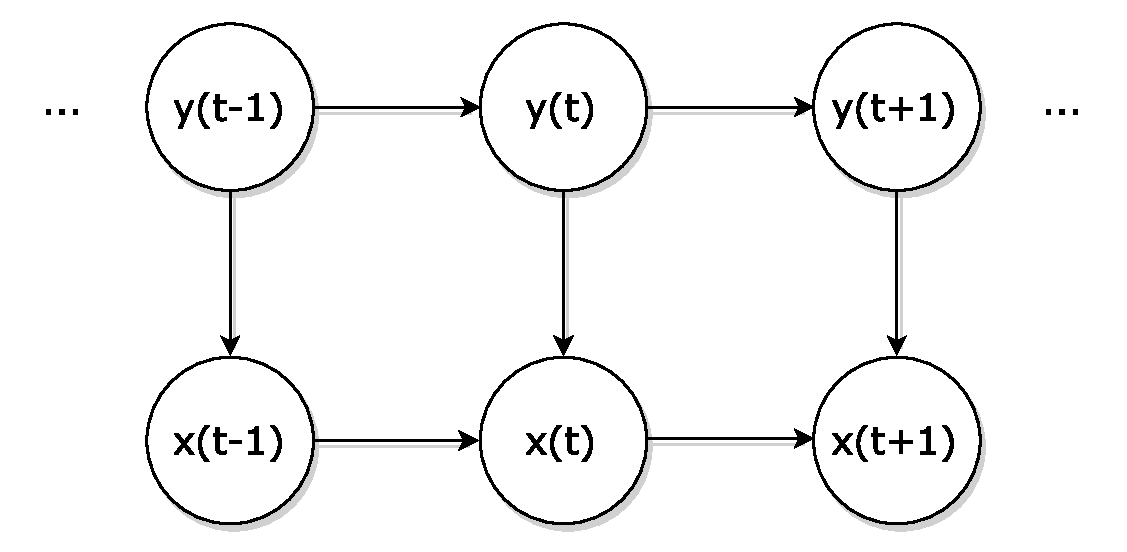
\includegraphics[width=4in]{Figures/HMM.pdf}
\caption{An illustration of the graphical structure of a Hidden Markov Model (HMM). The arrows indicate the dependencies running from dependee to dependent.}
\label{fig:HMM}
\end{figure}

We may build a HMM by first forming the joint probability distribution of the hidden state sequence and the observation sequence,

\begin{equation}
\p(\mathbf{x}, \mathbf{y}) = \p(\mathbf{x} | \mathbf{y}) \p(\mathbf{y}).
\label{eq:joint}
\end{equation}

Applying the chain rule and the dependency assumptions, we acquire,

\begin{equation}
\begin{aligned}
\p(\mathbf{x} | \mathbf{y}) &= \p(x_1|\mathbf{y}) \p(x_2|x_1, \mathbf{y}) ... \p(x_T|\mathbf{x}_{1:T-1}\mathbf{y}) \\
&= \p(x_1|y_1) \p(x_2|y_2) ... \p(x_T|y_T),
\end{aligned}
\label{eq:conditional}
\end{equation}

and,

\begin{equation}
\begin{aligned}
\p(\mathbf{y}) &= \p(y_1) \p(y_2|y_1) ... \p(y_T, \mathbf{y}_{1:T-1}) \\
&= \p(y_1) \p(y_2|y_1) ... \p(y_T, y_{T-1}).
\end{aligned}
\label{eq:prior}
\end{equation}

Combining \ref{eq:conditional} and \ref{eq:prior}, we may rewrite the factorisation of the HMM as,

\begin{equation}
\p(\mathbf{x}, \mathbf{y}) = \prod_{t=1}^T \p(y_t | y_{t-1})\p(x_t | y_t).
\label{eq:factorisedHMM}
\end{equation}

The probabilities $\p(y_t | y_{t-1})$ are known as \emph{transition} probabilities, and $\p(x_t | y_t) $ as \emph{emission} probabilities. These probabilities constitute the model parameters, $\theta = (\mathbf{A}, \mathbf{B}, \mathbf{I})$, where $\mathbf{A}$ is the $|S| \times |S|$ matrix of probabilities of transitioning from one state to another, $\mathbf{B}$ is the $|S| \times |O|$ matrix of probabilities of emitting an observation given an underlying hidden state, and $\mathbf{I}$ is the vector of probabilities of initial states. The model parameters must be precomputed\footnote{For example, the model parameters can be estimated through application of the Baum-Welch algorithm on an unsupervised training set.}. Now, given a sequence of observations, $\textbf{x}$, we may predict the hidden state sequence, $\mathbf{y}*$, by maximising the conditional distribution, $\p(\mathbf{y} | \mathbf{x})$. That is,

\begin{equation}
\textbf{y}* = \argmax_{\textbf{y}}\Bigg\{\prod_{t=1}^T \p(y_t | y_{t-1})\p(x_t | y_t)\Bigg\}.
\label{eq:argmax}
\end{equation}

The hidden state sequence prediction is chosen to be the one maximising the likelihood over all possible hidden sequences. This seemingly intractable problem may be solved in polynomial time using dynamic programming (see Section \ref{sec:viterbi}).

\section{Viterbi Algorithm}
\label{sec:viterbi}

The Viterbi algorithm is used to efficiently compute the most likely sequence, $\textbf{y}$, given an observation sequence, $\textbf{x}$. The algorithm can do this efficiently by working along the sequence from state to state, and choosing the transitions that maximise the likelihood of the sequence fragment. To show this we define, $v_t(s) = \max_{\mathbf{y}_{1:t-1}} \p(\mathbf{y}_{1:t-1}, y_t = s | \mathbf{x})$, that is, the most likely sequence from the first $t-1$ states, with the choice of state $s$ at time $t$. Thus, we may write,

\begin{equation}
\begin{aligned}
v_t(s) &= \max_{\mathbf{y}_{1:t-1}} \p(\mathbf{y}_{1:t-1} | \mathbf{x}) \p(y_{t-1}, y_t = s) \p(x_t | y_t = s) \\
&= \max_{\mathbf{y}_{1:t-1}} v_{t-1}(y_{t-1}) \p(y_{t-1}, y_t = s) \p(x_t | y_t = s), 
\end{aligned}
\label{eq:viterbi}
\end{equation}

and we may see the recursion. Once all states have been computed at time $t$, the maximum may be chosen and the algorithm proceeds to time $t+1$. Pseudocode for the Viterbi algorithm is given in Algorithm \ref{alg:viterbi} in Appendix \ref{AppendixA}. The algorithm must test all $|S|$ transitions from the previous state to each of the $|S|$ current states, and it does that for each of the $|T|$ steps in the sequence. Hence, the complexity of the algorithm is a workable $\mathcal{O}(T|S|^2)$.

\section{Forward-backward Algorithm}
\label{sec:fb}

Another key inference algorithm to sequence learning is the forward-backward algorithm, so called for its computation of variables in both directions along the sequence. It is another example of a dynamic programming algorithm and is used to compute the so-called \emph{forward-backward} variables, which are the conditional probabilities of the individual hidden states at each time step (that is, not the whole sequence), given the observation sequence and model parameters, namely, $\p(y_t = s | \mathbf{x}, \theta)$. These conditional probabilities have many useful applications, for example in the Baum-Welch algorithm for estimating model parameters, but also in the training of \emph{conditional random fields}, as we discuss in Section \ref{subsec:crfs}. We may write the forward-backward variables as,

\begin{equation}
\gamma_t(s) = \p(y_t = s | \mathbf{x}, \theta) = \frac{\alpha_t(s) \beta_t(s)}{\sum_{s' \in S} \alpha_t(s') \beta_t(s')},
\label{eq:fb}
\end{equation}

where the \emph{forward} variables, $\alpha_t(s) = \p(\mathbf{x}_{t+1:n}|y_t = s, \mathbf{x}_{1:t}) = \p(\mathbf{x}_{t+1:n}|y_t = s)$, and the \emph{backward} variables, $\beta_t(s) = \p(y_t = s, \mathbf{x}_{1:t})$. To derive the forward-backward algorithm we write, by the law of total probability,

\begin{equation}
\begin{aligned}
\alpha_t(s) &= \sum_{y_{t-1}} \p(y_{t-1}, y_t = s, \mathbf{x}_{1:t}) \\
& = \sum_{y_{t-1}} \p(y_t = s|y_{t-1}) \p(x_t|y_t) \p(y_{t-1}, \mathbf{x}_{1:t-1}) \\
& = \sum_{y_{t-1}} \mathbf{A}(y_{t-1}, s) \mathbf{B}(x_t, y_t) \alpha_{t-1}(y_{t-1})).
\end{aligned}
\label{eq:forward}
\end{equation}

Thus, we may see the recursion, as well as the way the forward variables will be computed, traversing the sequence in the forward direction with each forward variable of a given time a weighted product of those from the previous time. Likewise, for the backward variables, we may write,

\begin{equation}
\begin{aligned}
\beta_t(s) &= \sum_{y_{t+1}} \p(y_t = s, y_{t+1}, \mathbf{x}_{t+1:n}) \\
& = \sum_{y_{t+1}} \p(\mathbf{x}_{t+2:n}|y_{t+1}, x_{t+1}) \p(x_{t+1}, y_{t+1}|y_t = s) \\
& = \sum_{y_{t+1}} \beta_{t+1}(y_{t+1}) \mathbf{A}(s, y_{t+1}) \mathbf{B}(x_{t+1}, y_{t+1})).
\end{aligned}
\label{eq:backward}
\end{equation}

From Equations \ref{eq:forward} and \ref{eq:backward} comes Algorithm \ref{alg:fb} (Appendix \ref{AppendixA}). The complexity of the algorithm comes from noting that at each of the $T$ steps in the sequence (in either direction), we compute $|S|$ variables, involving a summation of $|S|$ products. Hence, like the Viterbi algorithm, the complexity of the forward-backward algorithm is $\mathcal{O}(T|S|^2)$.

\section{Maximum Entropy Classifiers}

Maximum entropy classifiers, also known as multinomial logistic regression, are a family of classification techniques.  A prediction is a discrete (categorical), scalar \emph{class}, rather than a class sequence as it is for HMMs. To build a model, we require a \emph{training set} consisting of a $N \times D$ matrix, $\mathbf{X}$, of $N$ training samples of dimension $D$\footnote{The dimensions of a model is synonymous with the model fields or features.}, as well as the $N$ corresponding classifications in the form of a vector, $\mathbf{y}$. A convex cost function known as a maximum log-likelihood function is constructed and subsequently optimised over the choice of model parameters, denoted $\boldsymbol\beta$. Thus, building a model is equivalent to solving a convex optimisation problem. A classification (prediction), $y*$, for an unseen data sample, $\mathbf{x}$, is made by employing these optimal model parameters in a linear function. The result is then passed through a non-linear \emph{logistic} function, denoted $\sigma$, to obtain a probability. Formally,

\begin{equation}
y* = \sigma(\boldsymbol\beta^T\mathbf{x}).
\label{eq:logisticprediction}
\end{equation}

The simplest form of maximum entropy classifier is binary logistic regression, where the number of classes to predict from is two, denoted $C_1$ and $C_2$. In this case, $\p(y_n = C_1|\mathbf{x}_n;\boldsymbol\beta) = \sigma(\boldsymbol\beta^T\mathbf{x}_n)$, and $\p(y_n = C_2|\mathbf{x}_n;\boldsymbol\beta) = 1 - \sigma(\boldsymbol\beta^T\mathbf{x}_n)$, where $C_1$ and $C_2$ are encoded as 0 and 1 respectively. Notice the probabilities sum to 1. Now, the log-likelihood can be expressed as,

\begin{equation}
\begin{aligned}
\log\p(\mathbf{y}|\mathbf{X}, \boldsymbol\beta) = \log\prod_{n=1}^N \p(y_n, \mathbf{x}_n)
&= \log\Bigg(\prod_{n:y_n = C_1}^N \sigma(\boldsymbol\beta^T\mathbf{x}_n) \prod_{n:y_n = C_2}^N 1 - \sigma(\boldsymbol\beta^T\mathbf{x}_n)\Bigg) \\
&=  \log\prod_{n = 1}^N \sigma(\boldsymbol\beta^T\mathbf{x}_n)^{y_i}(1 - \sigma(\boldsymbol\beta^T\mathbf{x}_n))^{1 - y_i}
\end{aligned}
\label{eq:logistic2}
\end{equation}

where $y_i \in \{0, 1\}$. We may then generalise to,

\begin{equation}
\begin{aligned}
\log\p(\mathbf{y}|\mathbf{X}, \boldsymbol\beta) = \log \prod_{n = 1}^N \prod_{c = 1}^C \mu_{nc}^{y_{nc}},
\end{aligned}
\label{eq:multinomial}
\end{equation}

where $y_{nc} = \mathbbm{1}_{\{y_n = c\}}$ and $y_n$ is a bit vector indicating the class of the $n$th sample. In this general, multinomial case, the probabilities are written, $\mu_{nc} = \frac{\exp(\boldsymbol\beta_c^T\mathbf{x}_n)}{\sum_{c' = 1}^C \exp(\boldsymbol\beta_c^T\mathbf{x}_n)}$, which are normalised to ensure they sum to 1, and $\boldsymbol\beta_c$ is part of a set of $C$ parameter vectors notated as $D \times C$ matrix, $\mathbf{B}$. From this we obtain a cost function,

\begin{equation}
\mathcal{L}(\mathbf{B}) = 
\log\p(\mathbf{y}|\mathbf{X}, \mathbf{B}) = \sum_{n=1}^N  \Bigg( \sum_{c = 1}^C y_{nc}\boldsymbol\beta_c^T \mathbf{x}^{(n)} \Bigg) - \log \Bigg( \sum_{c' = 1}^C \exp(\boldsymbol\beta_{c'}^T\mathbf{x}^{(n)})\Bigg).
\label{eq:logisticcost}
\end{equation}

Now we require an optimisation algorithm to solve for $\mathbf{B}$.

\section{L-BFGS}
\label{sec:lbfgs}

Convex optimisation problems may be solved numerically using variants of the method of greatest descent. These methods find the optimal model parameters by iteratively approaching a global minimum by taking steps opposite the gradient along the cost function hypersurface. The classic first-order gradient descent algorithm defines its iteration step to be,

\begin{equation}
\boldsymbol\beta^{k+1} = \boldsymbol\beta^{k} - \alpha\nabla\mathcal{L}(\boldsymbol\beta^{k}),
\label{eq:gd}
\end{equation}

where $\boldsymbol\beta$ is the vector of model parameters, $\alpha$ is the step size, and $\mathcal{L}$ is the cost function. Newton's method (also known as Iterated Reweighted Least Squares (IRLS)) takes a step in the direction minimising a second-order approximation of the cost function,

\begin{equation}
\boldsymbol\beta^{k+1} = \boldsymbol\beta^{k} - \alpha_k \mathbf{H_k}^{-1}\nabla\mathcal{L}(\boldsymbol\beta^{k}),
\label{eq:newton}
\end{equation}

where $\mathbf{H}$ is the $(D \times D)$ Hessian matrix of partial second derivatives. For smaller problems, these algorithms are adequate, however for models with millions of features, such as those that may be encountered in metadata extraction, smarter approaches are required. The \emph{Broyden--Fletcher--Goldfarb--Shanno} (BFGS) algorithm saves on the expensive computation of the Hessian by building up an approximation iteratively. The \emph{limited memory} BFGS (L-BFGS) algorithm makes further savings on the Hessian's \emph{storage}, and has come to be the standard learning algorithm for such problems. The L-BFGS algorithm is the tool of choice for many problems (\cite{murphy2012machine}) and is the algorithm we use in our analysis.

\section{Regularisation}

To avoid overfitting, we add a penalty to the cost function. This imposes a cost proportional to the size of the parameters for each dimension. Large parameters are therefore discouraged and this helps prevent the creation of complex models during training that do not fit test data well. This is equivalent to adding constraints to the optimisation problem. The two most common regularisation types are known as $l_1$ ad $l_2$ regularisation. The former imposes a \emph{Laplace} prior distribution on the parameters, and the latter a \emph{Gaussian}\footnote{A prior distribution in the Bayesian sense is the initial distribution of a variable taken independently.}. According to a probabilistic interpretation, this makes large parameters less likely and moderates their choices, and this is expressed in the cost function as the penalty. In our work, $l_2$ is the only type of regularisation compatible with L-BFGS (Section \ref{sec:lbfgs}).

\section{Conditional Random Fields}
\label{subsec:crfs}

Conditional Random Fields (CRFs) are a machine learning technique for making structured predictions. They are an improvement to the similar, Maximum Entropy Markov models (MEMM) (\cite{mccallum2000maximum}), which combine aspects of maximum entropy classifiers and Hidden Markov models (\cite{lafferty2001conditional}). They are a member of a class of structured sequence models called \emph{random fields}, which are part of a broader family known as \emph{graphical models}, including within it \emph{Bayesian networks}.

Classification over relational data can benefit greatly from rich features, that is, describing observed attributes of an observation beyond merely its identity (as with HMMs). Take for example the context of text processing, where we might consider describing a string token (observation) by non-lexical features such as by its capitalisation or punctuation. Furthermore, we may wish to model context-aware features that contrast a string token with its surroundings. However, the complexity of the interdependencies of such features will likely make their explicit modelling infeasible. With CRFs, we circumvent this problem by instead modelling the conditional distribution, $\p(\mathbf{y}|\mathbf{x})$, of the underlying graph structure, giving us free choice over features and, in so doing, \emph{implicitly} defining a distribution over $\mathbf{x}$ without having to model this distribution directly (\cite{sutton2006introduction}). Such a conditional model is called a \emph{discriminative} model, in contrast to a \emph{generative} model, whereby the joint probability distribution is modelled explicitly. If we wish to model the interdependencies in a generative model, we must either extend the model which may both be difficult and entail intractable solution algorithms, or we must simplify the model and thereby compromise model performance. Notice that modelling the conditional distribution is sufficient for classification, where the observation sequence is known. This freedom for rich feature engineering is what makes CRFs the current state-of-the-art in metadata extraction, where arbitrarily defined features often make for good indicators. One may be tempted to use a logistic regression and classify each part of a sequence separately, but this would fail to take into account the contextual relations between the entities. For example, in the metadata extraction of a bibiographic reference, it is more likely for a publication title to follow an author list, and for a journal name to follow a publication title. This is what we mean by structured sequence learning, where the data to predict exhibits interdependencies and are correlated.

When the graph structure of a CRF model is the same as for a HMM (Figure \ref{fig:HMM}), we have what is called a \emph{linear-chain} CRF. HMMs and linear-chain CRFs thereby form what is called a generative-discriminative pair. In the general case, where the graph structure is more complex, we have what is called \emph{skip-chain} CRFs. In this case the problem becomes far more complex, and we will not discuss these models here. A HMM may alternatively be expressed by the joint probability,

\begin{equation}
\p(\textbf{x}, \textbf{y}) = \text{exp} \Bigg\{
\sum_{i, j \in S}{
\lambda_{ij}F_{i,j}(y_t, y_{t-1}, x_t)
}
+
\sum_{i \in S}\sum_{o \in O}{
\mu_{io}F_{i,o}(y_t, y_{t-1}, x_t)
}
\Bigg\},
\label{eq:jointcrf}
\end{equation}

where the parameters $\lambda_{ij}$ are the transition probabilities and $\mu_{ij}$ are the emission probabilities. $F_{i,j}(y_t, y_{t-1}, x_t) = \sum_t^T\mathbbm{1}_{\{y_t = i\}}\mathbbm{1}_{\{y_{t-1} = j\}}$ is a \emph{feature function} used to activate the transition probabilities, and $F_{i,o}(y_t, y_{t-1}, x_t) = \sum_t^T\mathbbm{1}_{\{y_t = i\}}\mathbbm{1}_{\{x_{i} = o\}}$ for the emissions. The indicator functions activate the probabilities in accordance with the identity of the states and observations. Regardless, this formulation is equivalent to Equation \ref{eq:factorisedHMM}. With some notational abuse we can define the more compact expression,

\begin{equation}
\p(\textbf{x}, \textbf{y}) = \text{exp} \Bigg\{\sum_k{
\lambda_{k}F_{k}(y_t, y_{t-1}, x_t)
}\Bigg\},
\label{eq:jointcrfcompact}
\end{equation}

where $F_k$ is a general feature function and $\lambda_k$ a general feature weight. Now we may define the discriminative counterpart to this joint distribution, the linear-chain CRF,

\begin{equation}
\p(\textbf{y}|\textbf{x}) = \frac{\p(\textbf{x}, \textbf{y})}{\sum_{y'}{\p(\textbf{x}, \textbf{y}')}} = \frac{1}{Z(\mathbf{x})}\exp \Bigg\{\sum_k{
\lambda_{k}F_{k}(y_t, y_{t-1}, x_t)
}\Bigg\},
\end{equation}

where $Z(\mathbf{x}) = \sum_{y'}\exp \Big\{\sum_k{\lambda_{ij}F_{k}(y'_t, y'_{t-1}, x_t)}\Big\}$ is known as the partition function, ensuring probabilities sum to 1. Whereas HMMs model only the \emph{occurence} of a word, with conditional random fields we may choose $F_k$ to define arbitrarily complex features, describing rich information about a word, its attributes, and its context. Finally, we may define a cost function in the following way,

\begin{equation}
l(\theta) = \sum_{n=1}^N\sum_{t=1}^T\sum_{k=1}^K\lambda_kF_{k}(y_t, y_{t-1}, x_t) - \sum_{n=1}^N\log Z(\mathbf{x}^{(n)}) - \sum_{k=1}^K \frac{\lambda_k^2}{2\sigma^2},
\end{equation}

where $\theta = \{\lambda_k\}_{k=1}^K$. This is called penalised maximum log likelihood. The penalty term, $\sum_{k=1}^K\frac{\lambda_k^2}{2\sigma^2}$, imposes an $l_2$ regularisation on the solution parameters, $\theta$. However, according to (\cite{mccallum2000maximum}), varying the tuning parameter, $\sigma^2$ (the variance), by orders of magnitude has little effect on the outcome, a claim we corroborate in Chapter \ref{Chapter5}. This cost function represents a strictly convex function, solvable using numerical methods such as L-BFGS (see Section \ref{sec:lbfgs}). Forward-backward processing (Section \ref{sec:fb}) is performed at each iteration to compute the partition function, as well as the conditional probabilities resulting from deriving the partial derivatives required for gradient descent. Finally, the Viterbi algorithm (Section \ref{sec:viterbi}) is used to make a prediction with the trained model, that is, the best state sequence is found given the optimal parameter set found in training. A detailed exposition of this is given in (\cite{mccallum2000maximum}).

\section{Feature Functions}
\label{sec:featurefunctions}

In the simple HMM case (Equation \ref{eq:jointcrf}), there is a single feature function for each $(i, j)$ and $(i, o)$ pair. Furthermore, they are merely indicator functions that facilitate the activation of the transition and emission probabilities. In CRFs, however, we may define arbitrarily many and varied feature functions of the form $F_k(\mathbf{x}, y) = \sum_t^T f_k(\mathbf{x}, y)$, where $f_k$ is a (typically boolean) function describing one of several features about a token. Notice that while such a function is centered on a given token, that is, a specific element of $\mathbf{x}$, the function has access to the full vector $\mathbf{x}$, enabling the creation of context-aware features, combining information about a token with its neighbours. Further notice that the summation over the sequence is what enables instances (token sequences) of varying lengths to remain compatible with the model.

The form of the functions themselves, $f(\cdot)$, are known in Wapiti (Section \ref{sec:wapiti}) as \emph{templates}. It is in choosing these explicitly that we perform feature engineering. The literal feature functions, $\{f_k\}_{k=1}^K$, are formed by resolving the templates over the \emph{vocabularly} of features encountered in the extraction process prior to model training. In this way, we may see how model complexity depends on the diversity of the training set, and consequently, for smaller training sets, a model will have fewer feature functions. 

\section{Wapiti}
\label{sec:wapiti}

There are several open source software packages for the general purpose training and application of conditional random fields and related models. Wapiti (\cite{lavergne2010practical}), written in C, is the tool of choice for this project, given its compatibility with metadata extraction tool GROBID (Section \ref{sec:grobid}), its speed advantage over alternatives, and the recency of its development. It is developed by Thomas Lavergne at LIMSI, a computer science laboratory in Orsay affiliated with Paris-Sud University. It is capable, given sufficient memory, of training models with thousands of classes and billions of features. It implements several optimisation algorithms including L-BFGS (Section \ref{sec:lbfgs}) and stochastic gradient descent (SGD) and training is fully parallelisable. Wapiti has few drawbacks, but one is surely its lack of support for numeric features, as this curtails the scope for our feature engineering; any numeric-based idea must be discretised. Wapiti's main functions are training models and tagging. Training requires two inputs:

\begin{enumerate}
\item a feature template file, and;
\item a file of extracted features.
\end{enumerate}

The output of training is a model file. Tagging requires three inputs:

\begin{enumerate}
\item a feature template file;
\item a file of extracted features, and;
\item a trained model.
\end{enumerate}

The output of tagging is the file of extracted features appended with the classifications of each token. In the following we present samples of each of these files as they may look for a simple \emph{date} model for classifying dates into their \emph{day}, \emph{month}, and \emph{year} components.

\subsection{Feature Templates}
\label{subsec:featuretemplates}

Feature templates are the main access point for modelling with Wapiti. These files use a special syntax introduced by an older CRF engine, \emph{CRF++} (also supported by GROBID), allowing the operator to specify the form of the feature functions to be implemented in the model (see Section \ref{sec:featurefunctions}). The features are listed in a manner such as seen in Figure \ref{fig:featuretemplatefile}. The five features shown in Figure \ref{fig:featuretemplatefile} follow a similar format. The prefixes `U50', `U51' etc. are the unique identifiers of the macros. The `\%x' figures are wildcards for literal tokens. These macros are ultimatley expanded to feature functions when they are combined with the extracted features shown in Figure \ref{fig:extractedfeatures}. The indices given in square brackets indicate the row and column offset of the features considered. For example, `[0, 11]' in macro `U50' indiciates a row offset of 0, that is, pertaining to the current token, and a column offset of 11, pertaining to the $11th$ feature extracted in the feature extraction file (Section \ref{subsec:extractedfeatures}). Finally, macros `U53' and `U54', combine features from past and future tokens with the current one to make bigram features.

\begin{figure}
\centering
\begin{BVerbatim}
# Capitalization
U50:%x[0,11]
U51:%x[1,11]
U52:%x[-1,11]
U53:%x[0,11]/%x[1,11]
U54:%x[-1,11]/%x[0,11]
\end{BVerbatim}
\caption{Excerpt of capitalisation features templates or \emph{macros}.}
\label{fig:featuretemplatefile}
\end{figure}

\subsection{Extracted Features}
\label{subsec:extractedfeatures}

The extracted features file give the raw features for individual tokens. Note that feature templates may combine the raw features to make other, more complex features. Each line corresponds to a single token within each instance, and instances are grouped and separated by a line space. Figure \ref{fig:extractedfeatures} shows the features for a single instance of a date sequence, the string `4 August 1989'. The features for each token range from the original token (corresponding to a simple token indicator feature function such as in Equation \ref{eq:jointcrf}), to token prefixes \footnote{Prefixes are best seen for the `August token (`A', `Au', etc.); for the token `4', prefixes are identical to the original token.}, to information about capitalisation and punctation, and so on. Finally, we see the classifications of those tokens as `I-<day>', `I-<month>', and `I-<day>'.

\begin{figure}
\centering
\begin{BVerbatim}
4 4 4 4 4 4 LINESTART NOCAPS ALLDIGIT 1 0 0 NOPUNCT I-<day>
August august A Au Aug Augu LINEIN INITCAP NODIGIT 0 0 1 NOPUNCT I-<month>
1989 1989 1 19 198 1989 LINEEND NOCAPS ALLDIGIT 0 1 0 NOPUNCT I-<year>
\end{BVerbatim}
\caption{Features for a single date instance of three tokens: `4 August 1989'.}
\label{fig:extractedfeatures}
\end{figure}

\subsection{Models}

In Wapiti, a model consists of a large text file adhering to the following structure:

\begin{enumerate}
\item A list of the macros used (taken from the feature template file);
\item A list of classes modelled;
\item A list of expanded feature functions, and;
\item A list of corresponding (non-zero) weights, that is, the model parameters, represented in hexadecimal notation\footnote{This presumably to avoid numeric underflow.}.
\end{enumerate}

Of most interest are the expanded feature functions\footnote{Note the initial values of each line are simply the line lengths as a convenience to input processing.}, such as shown in Figure \ref{fig:expandedfeatures}. For example, feature function `u50' is a binary indicator for the capitalisation of the token. If the corresponding feature for this token is `NOCAPS', the result will be `1', otherwise, `0'. These functions are derivations of the macros defined in Figure \ref{fig:featuretemplatefile}.

\begin{figure}
\centering
\begin{BVerbatim}
10:u50:NOCAPS,
11:u51:INITCAP,
11:u52:INITCAP,
18:u53:NOCAPS/INITCAP,
18:u54:INITCAP/NOCAPS,
\end{BVerbatim}
\caption{Expanded feature functions deriving from capitalisation macros.}
\label{fig:expandedfeatures}
\end{figure}

\subsection{Training}

Training a model with Wapiti once all the input files have been prepared. The output given in Figure \ref{fig:output} shows the first six iterations of L-BFGS optimisation for training a \emph{date} model. In this case the number of instances (`nb train'), $N = 493$. The figure `nb blocks' refers to the number of feature functions per class that have come from combining extracted features (Section \ref{subsec:extractedfeatures}) and feature templates (Section \ref{subsec:featuretemplates}). The total number of feature functions (`nb features') is therefore this number multiplied by the number of classes, plus the number of transition functions, hence, $5816 \times 7 + 7 \times 6 = 40754$ features in total. Training a model to be sufficiently accurate generally takes hundreds or even thousands of iterations of L-BFGS.

\begin{figure}
\centering
\begin{BVerbatim}
* Initialize the model
* Summary
    nb train:    493
    nb labels:   7
    nb blocks:   5816
    nb features: 40754
* Train the model with l-bfgs
  [   1] obj=1688,58    act=16482    err=25,80%/50,91% time=0,08s/0,08s
  [   2] obj=1221,30    act=15580    err=19,11%/35,50% time=0,05s/0,12s
  [   3] obj=922,15     act=13869    err=17,20%/33,67% time=0,04s/0,17s
  [   4] obj=638,04     act=10845    err= 6,53%/15,21% time=0,04s/0,20s
  [   5] obj=478,72     act=10582    err= 5,68%/13,59% time=0,04s/0,24s
  [   6] obj=416,15     act=9926     err= 3,77%/ 9,53% time=0,04s/0,28s
\end{BVerbatim}
\caption{Output from training date model}
\label{fig:output}
\end{figure}
 
% Chapter 1

\chapter{Automatic Metadata Extraction} % Main chapter title

\label{Chapter3} % For referencing the chapter elsewhere, use \ref{Chapter1} 

\lhead{Chapter 3. \emph{Automatic Metadata Extraction}} % This is for the header on each page - perhaps a shortened title

%----------------------------------------------------------------------------------------

\emph{In this chapter we define the problem of automatic metadata extraction and discuss the methods by which the problem may be solved. Moreover, we introduce GROBID, the metadata extraction tool around which our work is based, and describe the cascade of CRF models it uses to solve the problem. Notably, we provide a comparison between GROBID and the existing solution for metadata extraction at CERN, `REFEXTRACT'.}

\section{Metadata Extraction}

Automatic metadata extraction (AME) has been referred to as `one of the hardest problems in document engineering'. In our work we are concerned with extraction for scientific articles that are usually (though not necessarily) in the form of a PDF document, as these predominate in the INSPIRE-HEP digital library. Nevertheless, the same techniques will be effective for books, theses, or may even have novel applications\footnote{Such as for segmenting cooking recipes, as reported in The New York Times (http://open.blogs.nytimes.com/2015/04/09/extracting-structured-data-from-recipes-using-conditional-random-fields/?\_r=0).}. At CERN, the problem has been partially solved, albeit in a rudimentary way, and also entails a lot of manual curation to complete the work. See Section \ref{subsec:refextract} for a comparison between this existing solution and GROBID, the leading tool for metadata extraction.

\emph{Metadata} refers to various information explicitly or implicitly contained in a scientific article. Perhaps the most important metadata for an article is that contained in the header, that is, the text at the front of a document, typically containing the title of the article as well as the names, affilations and often the contact details of the authors, concluding finally with the article abstract. As a general rule, this is tantamount to the text of the document falling before the first section of the body (usually called 'Introduction'), though as we find in Chapter \ref{Chapter4}, sometimes significant amounts of front matter is held in unexpected places. Other important types of metadata may be the references of the article, typically classified into fields such as publication title, authors, data of publication, and so on. Another potential metadata type is that of the document structure, its chapters and sections. All of these types are modelled by GROBID.

\emph{Extraction} could refer to either of two distinct concepts. First, it may be the parsing of a PDF document and extraction of plaintext and images. This in itself is a complex problem, and may involve machine learning techniques for OCR analysis, depending on the rendering of the document. Or, it may be the  \emph{classification} of document content into predefined categories. It is on the second idea that we are focused within this work. Indeed, GROBID addresses both of these points, but the first is merely a precondition for the analysis it is primarily concerned with, and it houses a third-party PDF to XML conversion tool, \emph{pdftoxml}, developed at Xerox Research Centre Europe (XRCE), to handle this (\cite{dejean2006system}).

\begin{figure}[!ht]
\subfloat[Header of article on CRFs.\label{subfig-1:header1}]{%
  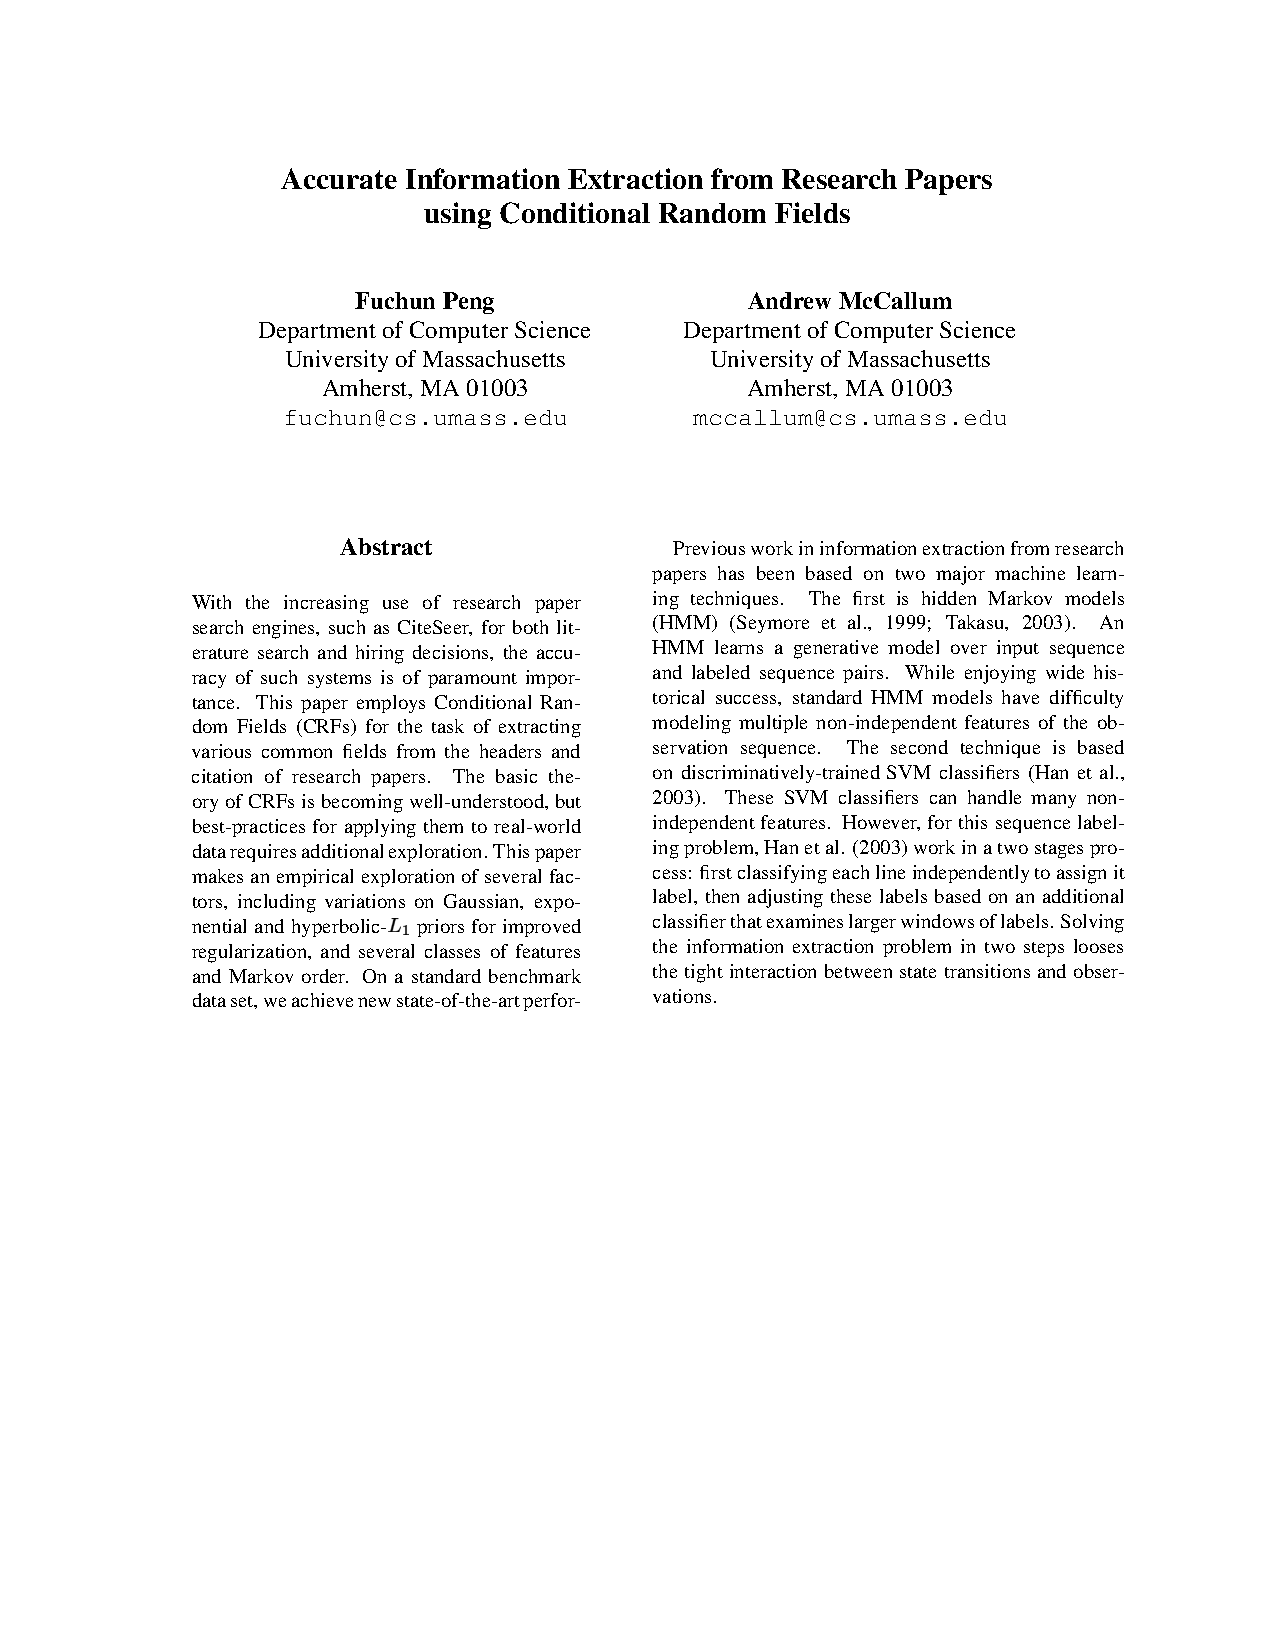
\includegraphics[width=0.45\textwidth]{Figures/header1.pdf}
}
\hfill
\subfloat[Header of a HEP paper.\label{subfig-2:header2}]{%
  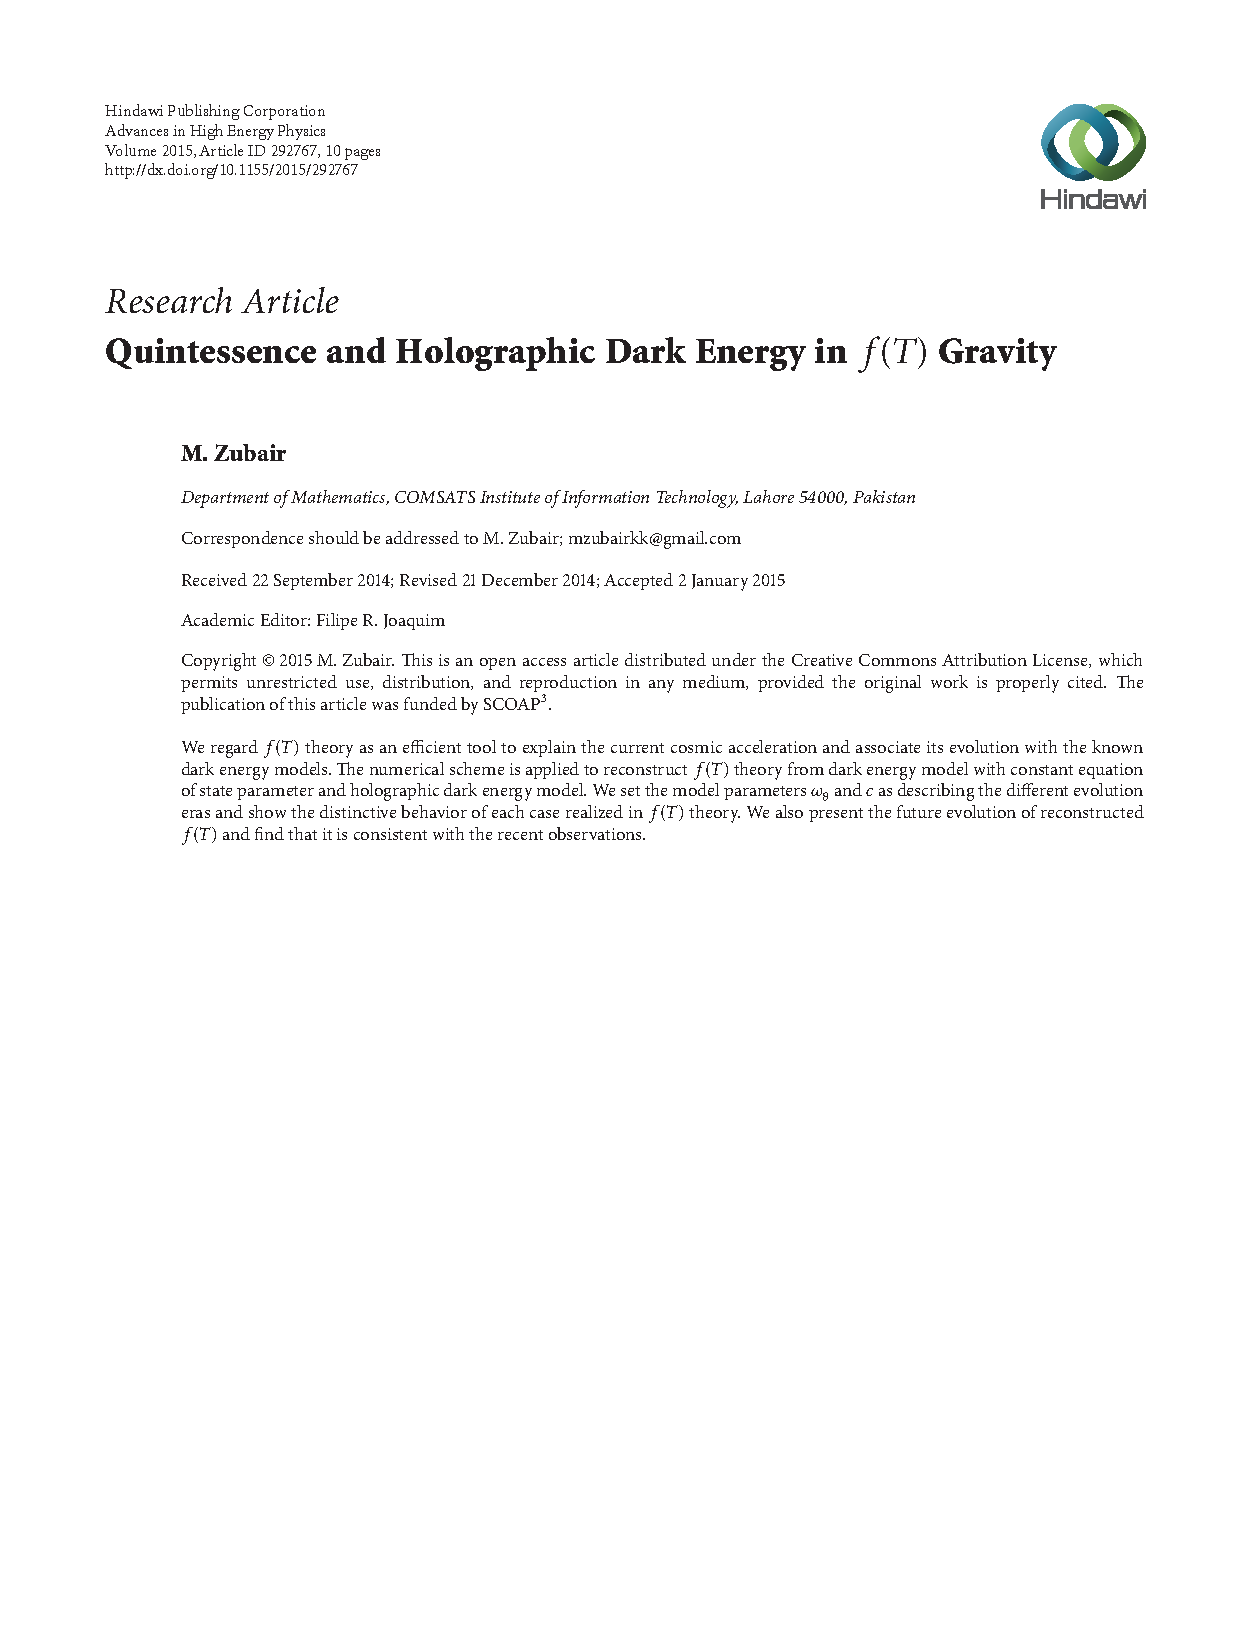
\includegraphics[width=0.45\textwidth]{Figures/header2.pdf}
}
\caption{Two differing header sections of articles from our dataset.}
\label{fig:headers}
\end{figure}

To appreciate the difficulty of automating such a task, consider Figure \ref{fig:headers}, contrasting the header sections of two articles from our dataset. Though the same sorts of information are present in both headers--title, author names, affilations, and document abstract--the arrangement and presentation of these fields are different, for example the sizing and placement of the document title, the juxtapositioning of authors (which are in variable in number) and author details, and labelling of the abstract block. Furthermore, the second header is more complete, in that it contains information not present in the other, for example copyright and publication details. The contents of a document header do not follow a predictable sequencing, making the problem hard, but are not entirely random, a condition that would render the problem impossible to solve. There is structure to a document, but it is likely infeasible to model deterministically. Therefore, we must look to probabilistic approaches, and accept that these will be error-prone.

\begin{figure}[!ht]
\center
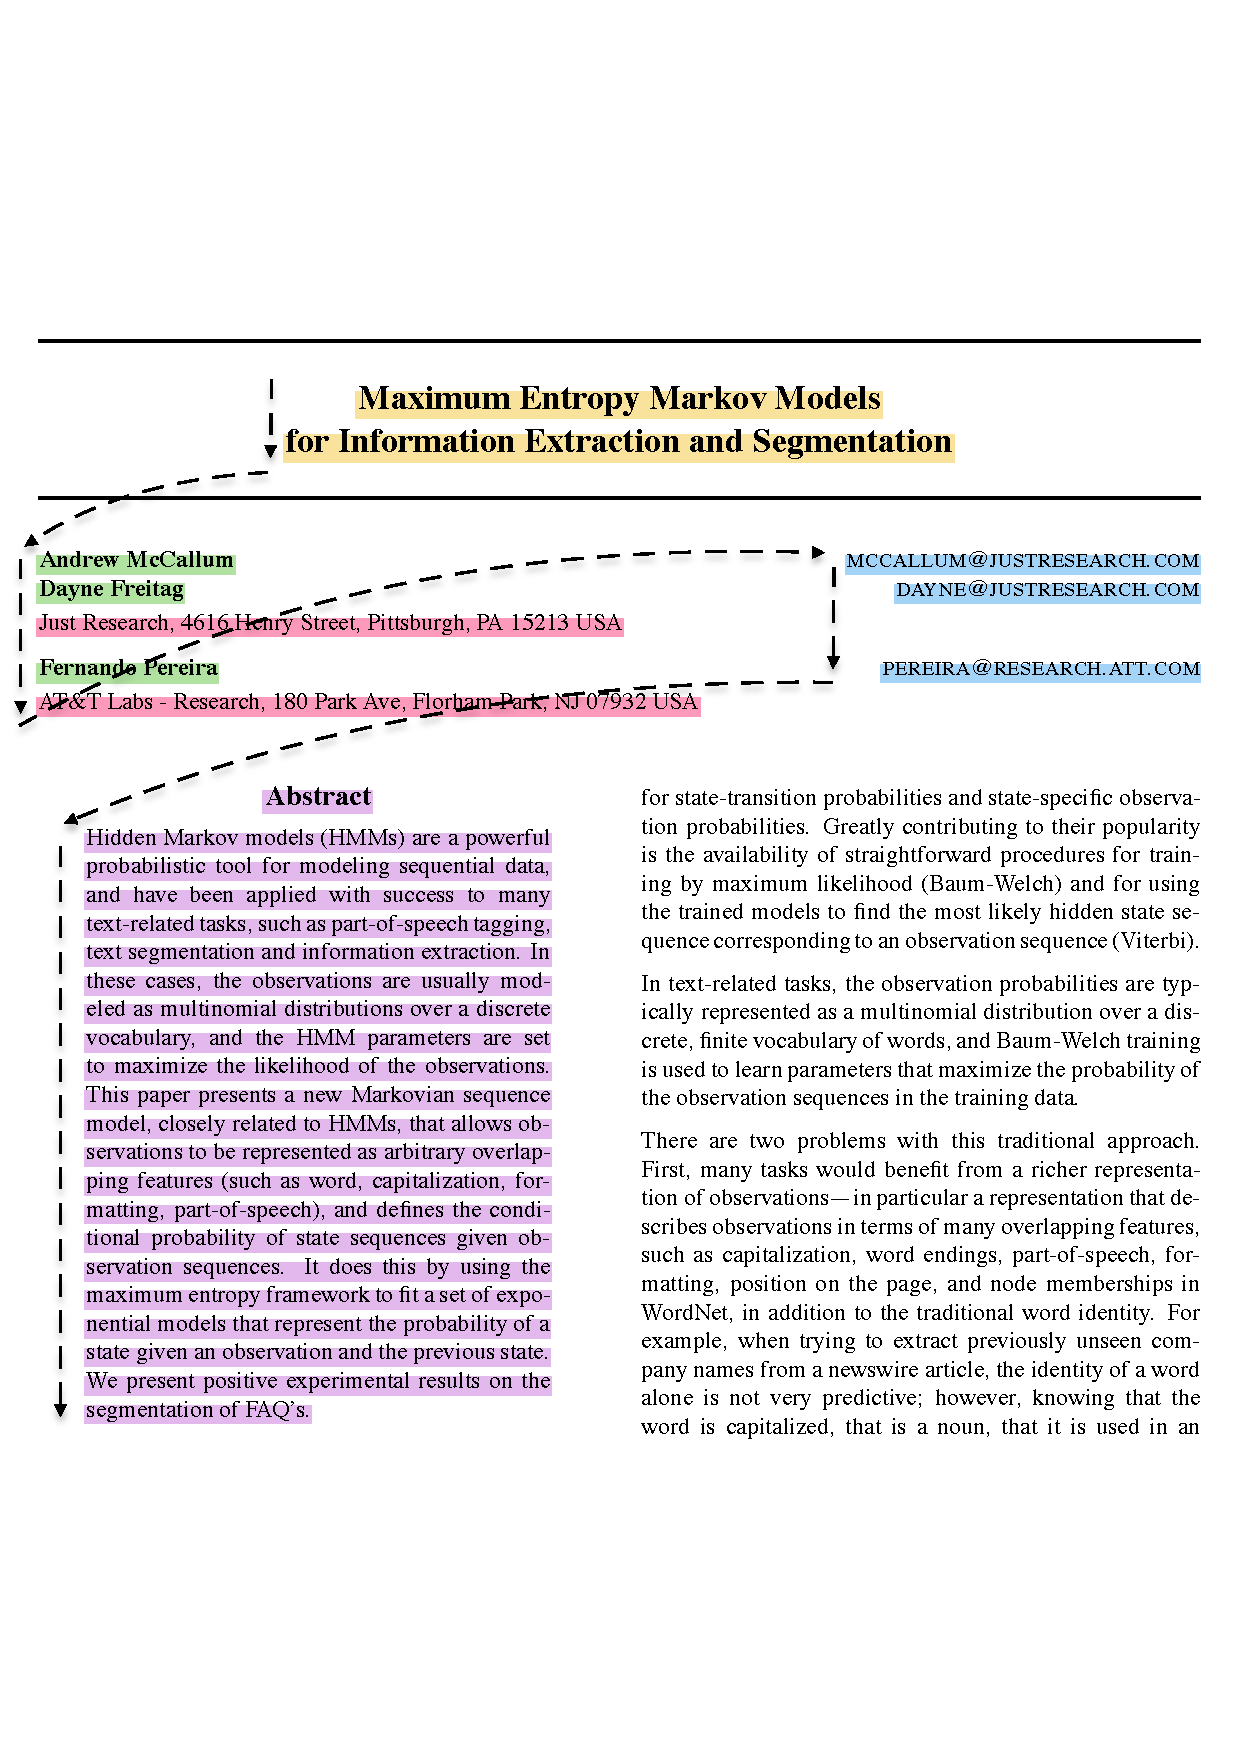
\includegraphics[width=\textwidth]{Figures/extraction.pdf}
\caption{An illustration of the interactions between Grobid and Wapiti for the two main functions of training and tagging.}
\label{fig:grobid}
\end{figure}

\section{Solution Methods}

A 2013 study of metadata extraction techniques \cite{lipinski2013evaluation} identified three fundamental methods for AME:

\begin{enumerate}
\item stylistic analysis;
\item knowledge base, and;
\item machine learning approaches.
\end{enumerate}

\emph{Stylistic analysis} refers to heuristic approaches to analysing physical characteristics of text font and layout. \emph{Knowledge base} methods rely on online repositories to cross reference extracted information. \emph{Machine learning} refers here either to the state-of-the-art conditional random fields, or to other approaches such as hidden Markov models or support vector machines. There is evidence to suggest that the best approach is a combination of the three methods, and the study admits software systems such as GROBID (Section \ref{sec:grobid}) do so. The study includes a comparison of the leading AME tools based on an ad hoc scoring system over fixed header extraction test data. GROBID performed best by a considerable margin, ahead of commercial applications Mendeley Desktop and ParsCit.

\section{GROBID}
\label{sec:grobid}
GROBID (GeneRatiOn of BIbliographic Data) \cite{lopez2009grobid} is an open-source (Apache license) Java-based tool for automatic metadata extraction. It has been in development by Patrice Lopez at the French Institute for Research in Computer Science and Automation (INRIA) since 2008. Grobid manages the training, evaluation and usage of a set of CRF models, each addressing a part of the information extraction of a scientific article. Higher level models such as the \emph{header}, \emph{segmentation}, and {reference-segmentater} models may applied directly to PDFs, while the other, more specific models, such as the Date model, operate only on plaintext inputs. Though they have much in common, the models vary in the labels they assign, the features they exploit, and, due to the varying size of the vocabulary (compare say, the number of possible month names to the number of possible author names), the size (dimensionality) of the models. Calling \texttt{processFullText} runs all available models on a batch of PDF documents. The output of training is a model, which takes takes the form of a text or binary file, depending on the engine. These models are then ``loaded'' at prediction time for the labelling of new documents. Some models are in practice not used independently, rather, they form part of a ``cascade'' of models that progressively address finer subcomponents of the classification problem. As shown in Figure \ref{fig:cascade}, reference extraction begins with segmentation models, which classify each line of a document, resulting in homogenous blocks of lines e.g. header, paragraph, figure, references. This information is then distributed to the other models, for example the Reference Segmentation model, which further breaks down the reference list into individual references. The Citation model then classifies the parts of each reference into classes, for example, date, affiliation, and author. Finally, the atomic subcomponents of these are classified by their respective models. Note that the citation branch of the hierarchy has the option of further cross-checking extracted references with the third-party CrossRef web service. Thus, the overall accuracy of the system is dependent on the combined accuracy of models.

\begin{center}
\begin{table}
\begin{tabular}{ | p{0.15\linewidth} | p{0.35\linewidth} | p{0.4\linewidth} |}
	\hline
	Model & Description & Labels \\ \hline
    Header & Extracts front matter & <title>, <author>, <affiliation>, <reference>, <submission>, <abstract>, <address>, <keyword>, <degree>, <pubnum>, <email>, <date>, <copyright>, <intro>, <web>, <note>, <phone>, <dedication>, <entitle>, <grant>, <date-submission> \\ \hline
	Affiliation address & Description & <institution>, <other>, <settlement>, <department>, <postcode>, <contry>, <marker>, <region>, <addrLine>, <laboratory>, <postbox>, <other>, <null> \\ \hline
	Name/ Header & Description & <forname>, <surname>, <marker>, <middlename>, <other>, <suffix>, <title> \\ \hline
	Name/ Citation & Description & <surname>, <forname>, <other>, <middlename> \\ \hline
	Citation & Description & <journal>, <volume>, <other>, <issue>, <pages>, <date>, <author>, <title>, <booktitle>, <location>, <pubnum>, <note>, <publisher>, <editor>, <institution>, <tech>, <web>, <issue> \\ \hline
	Date & & <other>, <day>, <month>, <year> \\ \hline
	Segmentation & The highest-level model in the architecture--primarily supplies the three models beneath it (header, fulltext and reference-segmenter) & <headnote>, <header>, <body>, <page>, <references>, <footnote>, <cover>, <acknowledgement>, <annex> \\ \hline
	Reference-Segmenter & Description & <label>, <reference>, <other> \\ \hline
	Fulltext & Description & <section>, <paragraph>, <citation\_marker>, <other>, <table\_marker>, <figure\_marker>, <figure\_head>, <trash>, <figDesc>, <equation>, <item> \\ \hline
\end{tabular}
\caption{We have here excluded the Patent, Entities, and E-book models as these are experimental models not currently used by Grobid. Of the models listed, we will be focusing on Header, probably Segmentation, and perhaps Reference-Segmenter and Citation also. This is because these are likely to require special training and configuration for HEP papers. Others such as Name and Date are unlikely to improve with training on HEP papers.}
\label{fig:featurelist}
\end{table}
\end{center}

Both training and evaluation are performed on sets of XML documents following the Text Encoding Initiative (TEI) standard for representing electronic texts (http://www.tei-c.org/index.xml). This is also the output format for prediction, so there is consistency between input and output formats. It may appear paradoxical to \emph{evaluate} on well-structured data, when the tool is ultimately intended to operate on unstructured PDF documents, that is, at prediction time. However, with closer inspection of the source code, an equivalence can be seen between:

Both approaches yield the same input data for the CRF engine, and so evaluation is in fact equivalent to prediction, despite the initial difference in input formats. Figure \ref{fig:traininput} shows an excerpt from an input file to the CRF engine for training. These features are for inputs ``January 1994'' and ``July 1996'', for training the Date model. The features range from token identity, to a variety of prefixes and punctuation features. It should be noted that OCR information is only used in higher level models, that is, the Header and Segmentation models. The input for lower-level models such as Date is plaintext, and so features are typically simple, but dictionary-based features, where information about a token is referenced in a dictionary resource within Grobid, are also used. Note the features shown are only those pertaining to the token itself. The full range of features (including those involving concatenations of the token's neighbours etc.) are defined by a set of feature templates. The feature templates for each model are contained in a separate file. An excerpt of this is shown in Figure \ref{fig:template}. These are given as a separate input to the CRF engine, and it is with these that the engine constructs all feature functions for the model. It is therefore vital that the feature extraction, which is generated by Grobid, is aligned with the template file, which is manually configured by the developer. As depicted in Figure \ref{fig:flow}, there is a strong coupling between these two parts of Grobid. The excerpt shown is from the Wapiti model, but the notation is the same for CRF++, which first standardised the syntax. This subset of five feature templates capture information about the capitalisation of a token and its neighbours. The notation has the structure, [identifier]:[\%x][row, col], where row is the offset from the current token, and col indicates the feature index. Thus, ``U50:\%[0,11]'', denotes that the feature template identified as ``U50'' takes the 11th feature for the current token (0 offset). This feature will be equal to 1 if a token is capitalised, and 0 otherwise. ``U52:\%[-1,11]'' indicates the same thing, but based on the capitalisation of the \emph{previous} token. ``U54:\%x[-1,11]/\%x[0,11]'' is a binary function for detecting the capitalisation of the current \emph{and} the following token.

\subsection{Evaluation}

Training may be done with a split defined by the developer, which Grobid will use to set aside a proportion of the training data for evaluation. The evaluation of a model produced by training follows identical procedures, preparing the same input data. The output, however, is not a model but a the input data with labels. Grobid compares its predictions with the ground truth and outputs \emph{precision}, \emph{accuracy} and \emph{F1 scores} as performance indicators, at the token, field, and instance levels. A token refers to a single contiguous string of characters (without spaces), a field is a block of contiguous tokens, and an instance is an entire document. Accuracy of an instance is therefore judged by the correctness of all tagging for the whole document, a difficult thing to achieve without any mistakes.

\subsection{Prediction}

Figure \ref{fig:flow} shows the flow of information from input to output, as well as the relationship between training and prediction. When it comes to labelling (prediction), the starting point is a PDF document. With a third-party tool, pdftoxml, this is transformed into an XML file containing OCR information (font, style, orientation) for every token in the document. This information is stored in LayoutToken objects within Grobid. These tokens are arranged into blocks and features are extracted as they were for training and evaluation. Excepting the absence of tokens, the input is the same. The model created in the training phase is first loaded, and then the EngineTagger calls the CRF engine to label the inputs. Unlike for training, the feature template file is not required, as these have already been absorbed into the model file. After processing, Wapiti returns the same file with tags inserted. Grobid then further processes this information to transform it into the final TEI format.

\subsection{Other Functionality}

In addition to the above, Grobid provides a means of producing training sets semi-automatically. This consists of applying the existing models on the training set to produce the XML inputs. Of course, each field must be checked against a ground truth and errors corrected before it is used as a training set. We intend to use this functionality to generate training data for benchmarking Grobid on HEP papers.

\begin{figure}[!ht]
\center
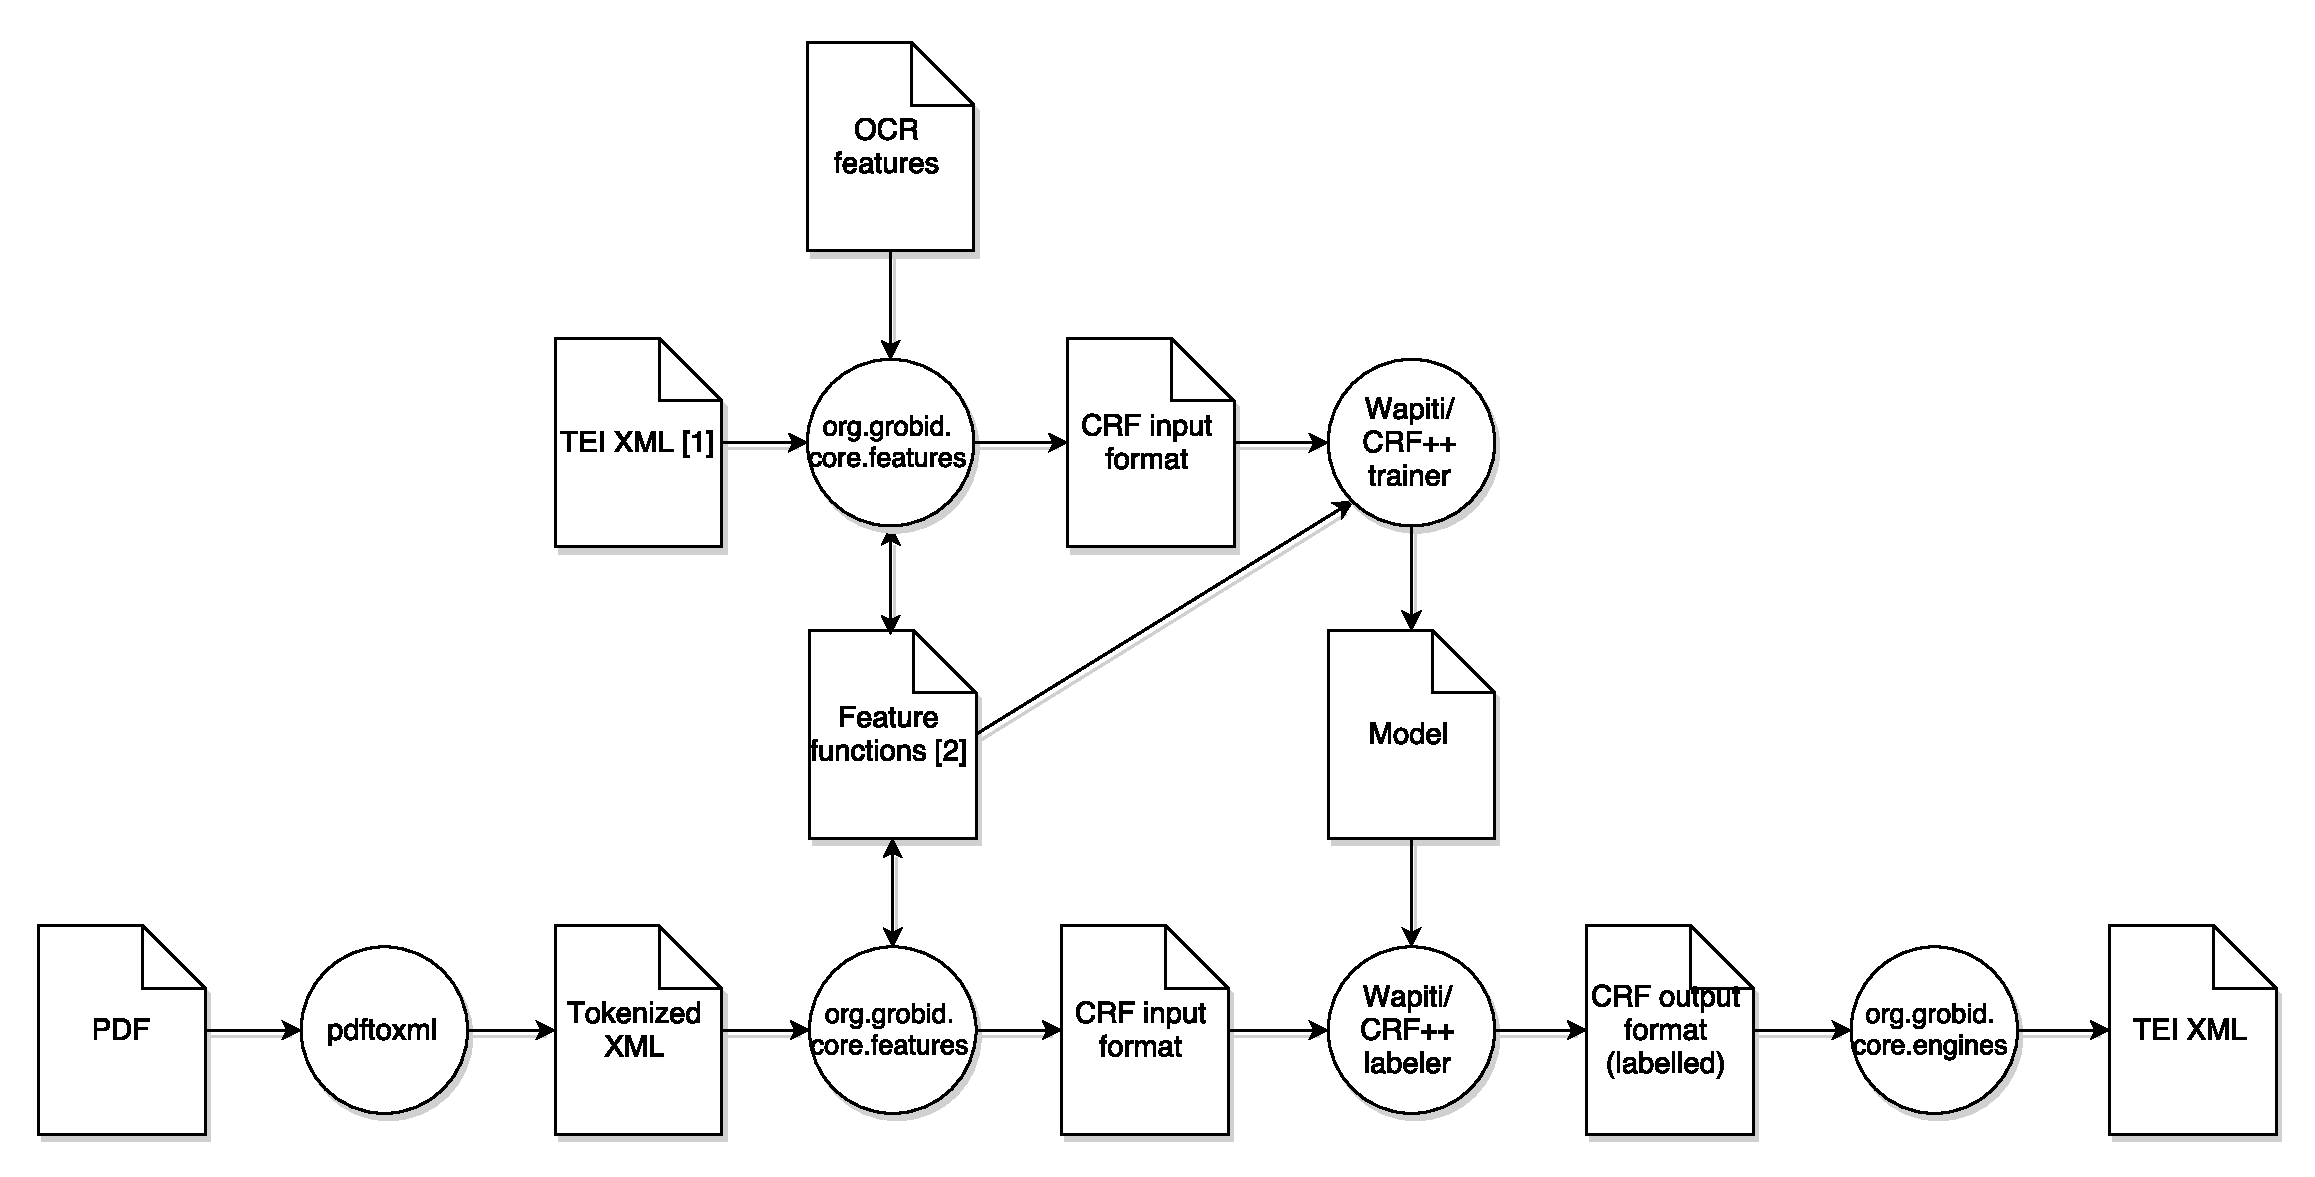
\includegraphics[width=\textwidth]{Figures/grobid.pdf}
\caption{An illustration of the interactions between Grobid and Wapiti for the two main functions of training and tagging.}
\label{fig:grobid}
\end{figure}

\begin{figure}[!ht]
\center
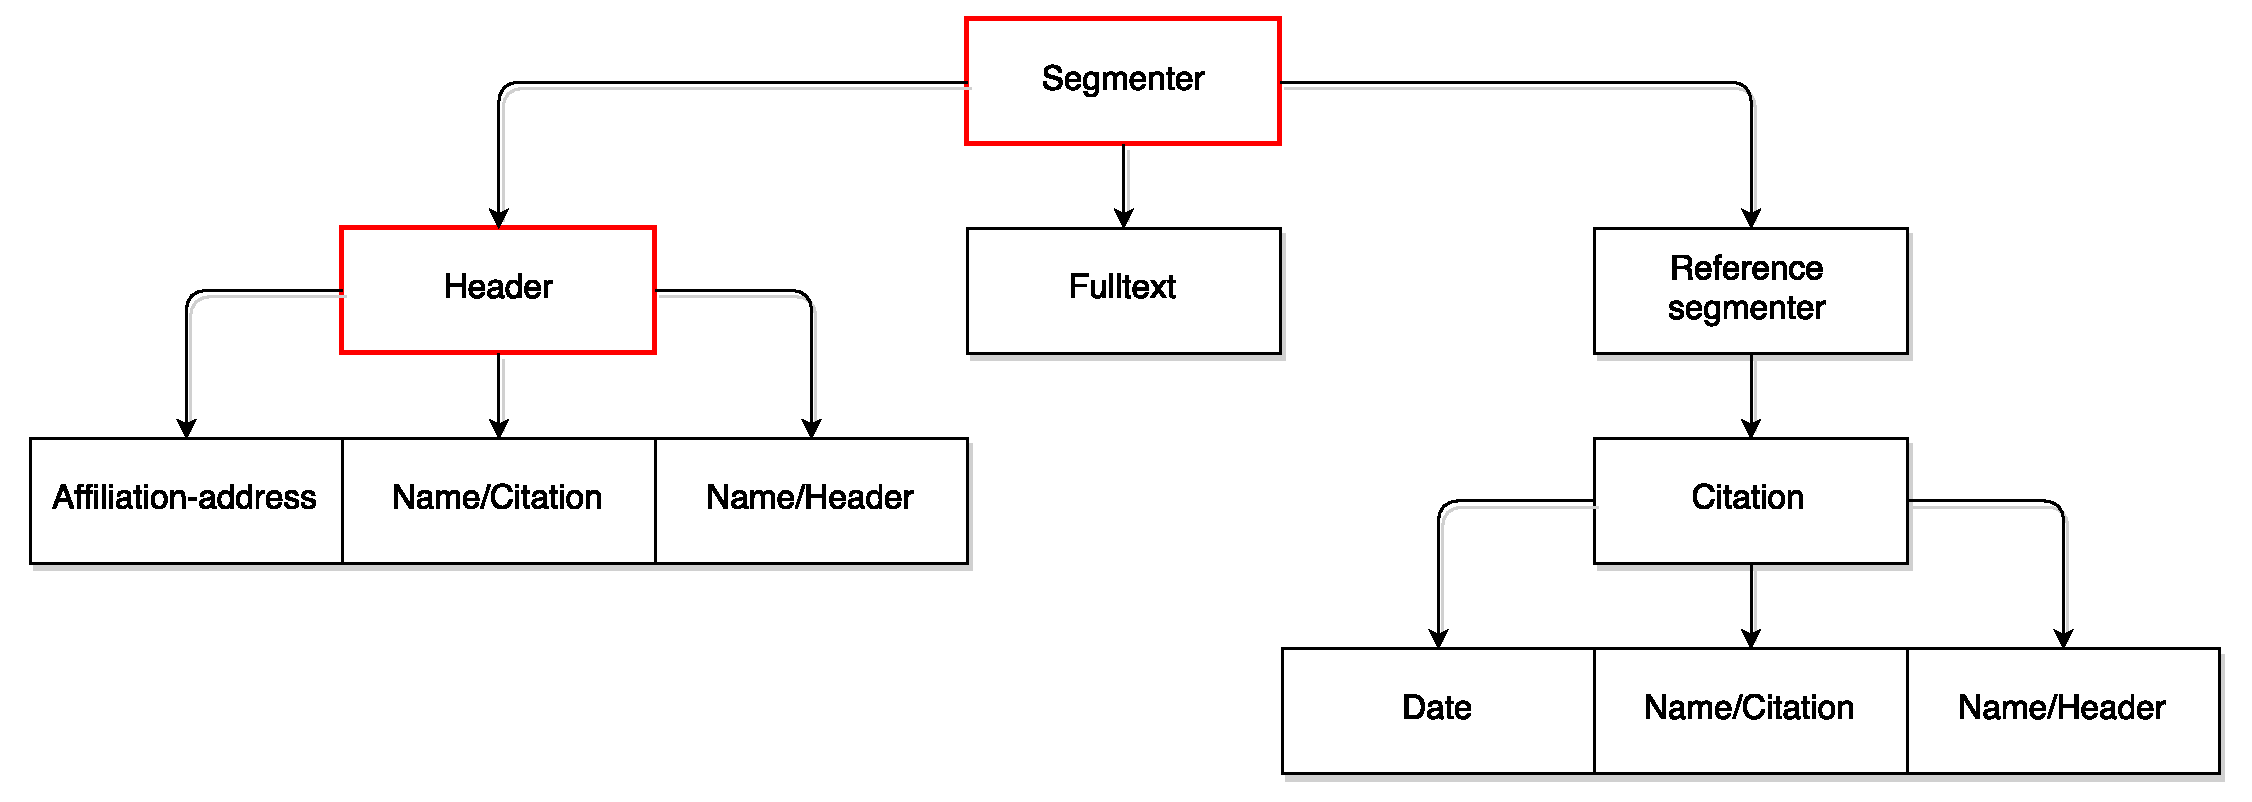
\includegraphics[width=\textwidth]{Figures/cascade.pdf}
\caption{The models of Grobid are organised into a cascade, where each part of a document is classified in increasingly greater detail.}
\label{fig:cascade}
\end{figure}

\subsection{Comparison with REFEXTRACT}

By way of a benchmarking evaluation for GROBID, we compare it with REFEXTRACT, the existing solution. As mentioned earlier, this existing tool is incomplete and greatly lacking in the . It is capable only of retrieving references\footnote{A comparatively easy task; GROBID's citation model usually performs at a significantly higher accuracy than, say, the header model.}, and the classification itself is quite basic. Since the modelling of reference fields differs between the two, a comparison is difficult to make. A comparison will at least be indicative, however, and we are able to make reasonable comparisons on the most important fields. The dataset for the comparison consists of 60 articles coming from the SCOAP$^3$ online repository\footnote{Scoap$^3$ (Sponsoring Open Consortium for Open Access Publishing in Particle Physics) is an open access digital library hosted at CERN, backed by an international partnership of research institutions.}.

Unlike REFEXTRACT, GROBID requires two separate models to classify the citations of a given article: the reference-segmenter and citation models\footnote{Strictly speaking, there is another model, (full) Segmentation, above the reference-segmenter, and so citation accuracy depends on this also. But because one focus of our work is to improve this model, we accept this omission.}. The former . Therefore, the accuracy of the citation model is ultimately subject to the accuracy of the refernence block inputs supplied to it. The citation model, unlike

\label{subsec:refextract}
\begin{table}[h]
\begin{center}
\begin{tabular}{|c|cccc|}
\hline
label		&accuracy	&precision	&recall		&f1 \\
\hline
<label>		&99.96		&100		&99.2		&99.6\\
<reference>		&99.96		&99.96		&100		&99.98\\
\hline
(micro average) & 99.96		&99.96		&99.96		&99.96	\\
(macro average) &	99.96 & 99.98	& 99.6 & 99.79	\\
\hline
\end{tabular}
\caption[Table caption text]{Evaluation results for reference segmentation}
\end{center}
\end{table}

\begin{table}[h]
\begin{center}
\begin{tabular}{|c|cccc|cccc|}
\hline
engine &  \multicolumn{4}{c}{GROBID} & \multicolumn{4}{c}{REFEXTRACT}\\
\hline
label & accuracy & precision & recall & f1 & acc. & prec. & rec. & f1\\
\hline
<author>	&	99.85	&	99.68	&	99.75	&	99.72 	& 98.33	&	100	&	92.22	&	95.95	\\
<title>	&	99.59	&	98.87	&	99.25	&	99.06 	& 94.89	&	100	&	71.75	&	83.55	\\
<journal>	&	98.84	&	88.87	&	93.98	&	91.35 	& 97.12	&	100	&	46.78	&	63.74	\\
<volume>&	99.95	&	99.07	&	98.15	&	98.6 		& 98.36	&	0	&	0		&	0	\\
<issue>	&	99.93	&	100		&	94.63	&	97.24	 & 98.87	&	0	&	0		&	0	\\
<pages>	&	99.75	&	93.51	&	99.45	&	96.39 	& 97.26	&	0	&	0		&	0	\\
<date>	&	98.39	&	57.39	&	98.31	&	72.47 	& 98.88	&	100	&	37.55	&	54.6	\\
<pubnum>&	98.71	&	100		&	12.96	&	22.95 	& 98.77	&	0	&	0		&	0	\\
<note>	&	99.4	 	&	43.75	&	35		&	38.89 	& 99.55	&	0	&	0		&	0	\\
<publisher>&	99.81	&	63.46	&	94.29	&	75.86 	& 99.73	&	0	&	0		&	0	\\
<location>&	99.81	&	86.32	&	91.11	&	88.65 	& 99.32	&	0	&	0		&	0	\\
<institution>&	99.78	&	25		&	25		&	25 		& 99.88	&	0	&	0		&	0	\\
<booktitle>&	98.7		&	55.56	&	41.67	&	47.62 	& 98.82	&	0	&	0		&	0	\\
<web>	&	99.64	&	51.85	&	100		&	68.29 	& 99.68	&	0	&	0		&	0	\\
<editor>	&	99.93	&	100		&46.67		&	63.64 	& 99.89	&	0	&	0		&	0	\\
<tech>	&	99.95	&	83.33	&	50		&	62.5 		& 99.92	&	0	&	0		&	0	\\
\hline
(micro average) & 99.5	&	93.63	&	94.77 	&	94.19 & 98.7	&	100	&	63.47 	&	77.65	\\
(macro average) & 99.5	&	77.92	&	73.76	&	71.76 & 98.7	&	25	&	15.52	&	18.62	\\
\hline
\end{tabular}
\caption[Table caption text]{Evaluation results for citations}
\end{center}
\end{table}

% Chapter 1

\chapter{Implementation and Data} % Main chapter title

\label{Chapter4} % For referencing the chapter elsewhere, use \ref{Chapter1} 

\lhead{Chapter 4. \emph{Implementation and Data}} % This is for the header on each page - perhaps a shortened title

\emph{In this chapter we present our work, which centers around 66 cross-validated feature engineering experiments including a baseline evaluation. The work is divided into four components: first, the procurement of HEP training data with which to perform the experiments; then, the extensions made to GROBID to facilitate our feature engineering and evaluations; next, the pipeline assembled for automating the experimentation; and finally, the different categories of feature engineering, and our reasons for choosing them.}

\section{Objectives}

As articulated in Chapter \ref{Chapter3}, GROBID manages a hierarchy of models that propagates classified information from top to bottom in a cascade. Our objectives are therefore to enhance some models within the cascade for HEP papers. It does not, on the other hand, make sense to attempt to improve all models. After all, we may assume a HEP \emph{date} is no different from dates printed in other scientific papers. Aside for feature engineering, it is hard to imagine improving performance of these models which exemplary. The same goes for names, and with little exception\footnote{It is in fact true that HEP collaborations feature in isolated references in HEP papers (see Section \ref{sec:futurework}).}, reference lists and their contents. Undoubtedly, the models with the most promising scope for improvement are the \emph{header} and \emph{segmentation} models. It is these models that address the parts of an article most distinct in HEP papers. In particular, some physical journals have recurrent styles and formats for headers sections that are distinct from others publishers. In addition, the vocabularly of a physics headers will be distinct from that papers from other branches of sceience. These should be trained for and additionally engineered for, for example through the use of dictionary-based features (see Section \ref{sec:dicts}). Thus, the \emph{header} model may be improved for a number of reasons, including:

\begin{enumerate}
\item physics publishers present a unique format not found in CORA papers;
\item scientific collaborations as seen in HEP papers are not modelled as a header class by vanilla GROBID, and;
\item discontinuous header data (see Figure XXX), which may contain substantial front matter is by default neither trained nor modelled for.
\end{enumerate}

The \emph{segmentation} model may also be improved for a number of reasons:

\begin{enumerate}
\item discontinuous header data (see Figure XXX), which may contain substantial information is neither trained nor modelled for;
\item HEP collaborations entail long author lists and affiliation lists, often disjoint from the main header section, which are neither trained nor modelled for, and;
\item the dataset is small (we more than double it in Section \ref{sec:data}).
\end{enumerate}

Note that the \emph{segmentation} model is the parent model of the entire cascade, and therefore any improvement to it will benefit all other models at prediction time. Aside from being the root of the cascade, the \emph{segmentation} model is special in that it models. A comparison is given in Table \ref{table:headervssegmentation}. We are mindful of this distinction as we go about our feature engineering.

\begin{table}[h]
\begin{center}
\begin{tabular}{|c|c|c|}
\hline
Model & Token & Instance \\
\hline
Header & Character string & Header section \\
\hline
Segmentation & Full line & Full document \\
\hline
\end{tabular}
\caption[Comparison of token and instance ]{Evaluation results for reference segmentation}
\label{table:headervssegmentation}
\end{center}
\end{table}

Our focus is therefore on the two models, \emph{header} and \emph{segmentation}. We therefore require two separate training sets of HEP papers, one for each model. Incidentally, both models require that for each [paper we produce a TEI representation and a \emph{raw} file of extracted features, as explained in Section \ref{sec:grobid}.

\section{Data Acquisition}
\label{sec:data}

At the recommendation of an INSPIRE-HEP library curator, we selected a set of articles deemed to be a representative sample of the database. It contains the following varieties of papers:

\begin{enumerate}
\item conference papers (no DOI);
\item conference papers (with DOI);
\item general papers;
\item miscellaneous papers (including non-English language), and;
\item collaboration papers.
\end{enumerate}

This totalled 191 papers\footnote{Originally this numbered in excess of 200, but certain papers could not be parsed by \emph{pdf2xml}.}, however according to our adjudications, we additionally removed articles deemed to be unsuitable for training, such as books. The starting point for generating training data is to apply the existing, default models of GROBID on the new dataset of PDF papers. For \emph{segmentation} training data, the command for this is \texttt{createTrainingSegmentation}. 

In Sections \ref{subsec:cora}, \ref{subsec:hepdatasetheader}, and \ref{subsec:hepdatasetsegmentation}, we detail the mixture of data we have assembled.

\begin{table}[h]
\begin{center}
\begin{tabular}{|c|c|c|}
\hline
Model & HEP & CORA \\
\hline
Header & 157 & \textbf{2506} \\
\hline
Segmentation & \textbf{169} & 125 \\
\hline
\end{tabular}
\caption[Number of training instances for each model from each dataset.]{Number of training instances for each model from each dataset.}
\label{table:headervssegmentation}
\end{center}
\end{table}

\subsection{CORA dataset}
\label{subsec:cora}
The CORA (ACRONYM) dataset is a substantial dataset of some 2506 header instances. It is popular in metadata extraction studies, as creating custom training data is a stupendously time-consuming task, and has come to be a sort of standard (\cite{Peng04accurateinformation}). From One of the questions we ask in Section \ref{sec:results} is therefore, what 

\begin{enumerate}
\item the dataset is small (we more than double it in Section \ref{sec:data})
\item the dataset is small (we more than double it in Section \ref{sec:data})
\item the dataset is small (we more than double it in Section \ref{sec:data})
\item the dataset is small (we more than double it in Section \ref{sec:data})
\end{enumerate}

Despite the overall quality of the dataset, we did encounter some small mistakes, as do (\cite{Peng04accurateinformation})

\blockquote{The \emph{note} field is the one most confused with others, and upon inspection is actually labeled inconsistently in the training data.}

\subsection{HEP dataset - Header}
\label{subsec:hepdatasetheader}

We were therefore able to experiment with combining the two datasets of HEP papers, as well as subsampling the CORA dataset to see . After all, in spite of common wisdom that increasing the amount of training data will increase generalisation and model performance, it is not clear what effects combining different ground truths, namely CORA and HEP, will have. One may imagine that generalising over a hybrid dataset might construct a misleading model when it comes to evaluate on a pure HEP dataset, especially when the CORA set dwarfs our HEP one. Therefore one of our research questions is whether such a mixture is beneficial, and we experiment with different CORA sample sizes in Section \ref{Chapter5}.

\begin{figure}
\centering
\begin{tabular}{cc}
\subfloat[Headnote]{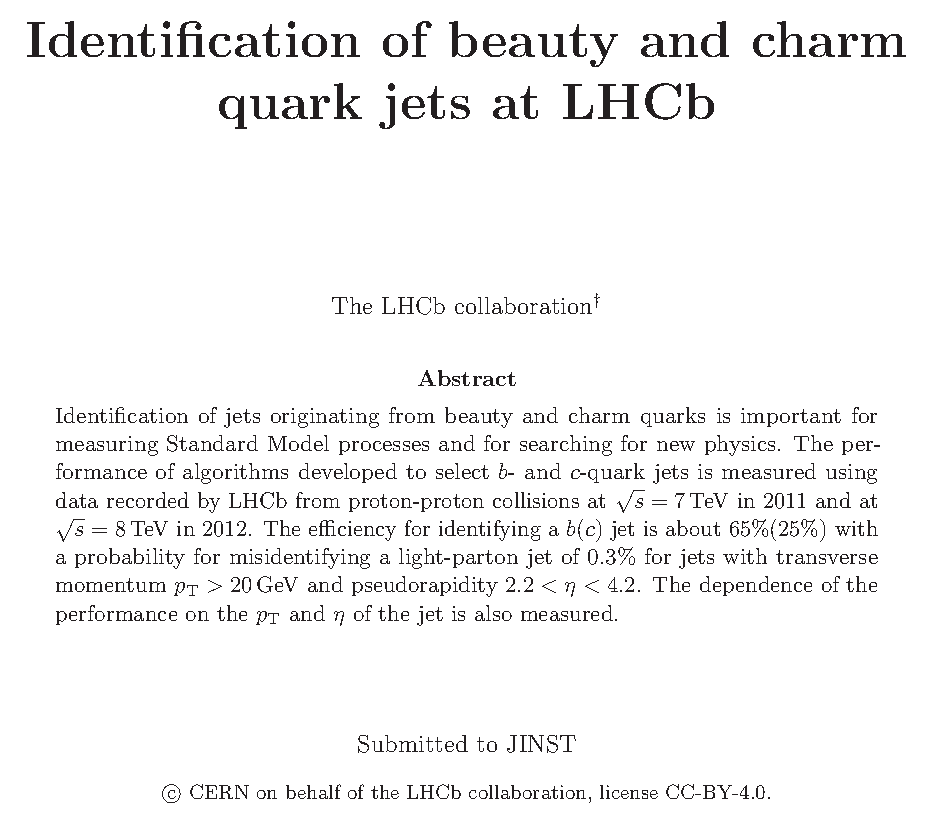
\includegraphics[width=0.45\textwidth]{Figures/collaboration.pdf}}&
\subfloat[Page number]{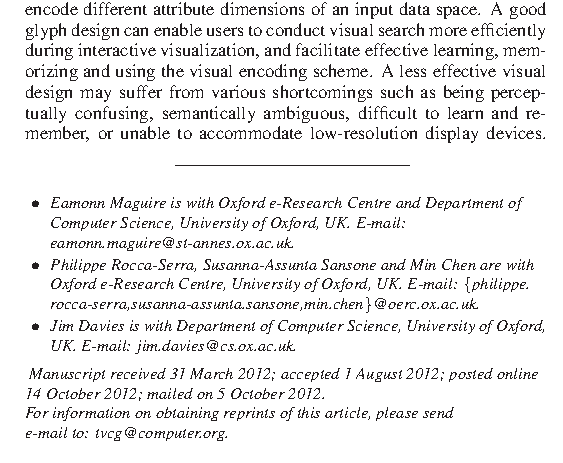
\includegraphics[width=0.45\textwidth]{Figures/eamonn.pdf}} \\
\subfloat[Body (formula)]{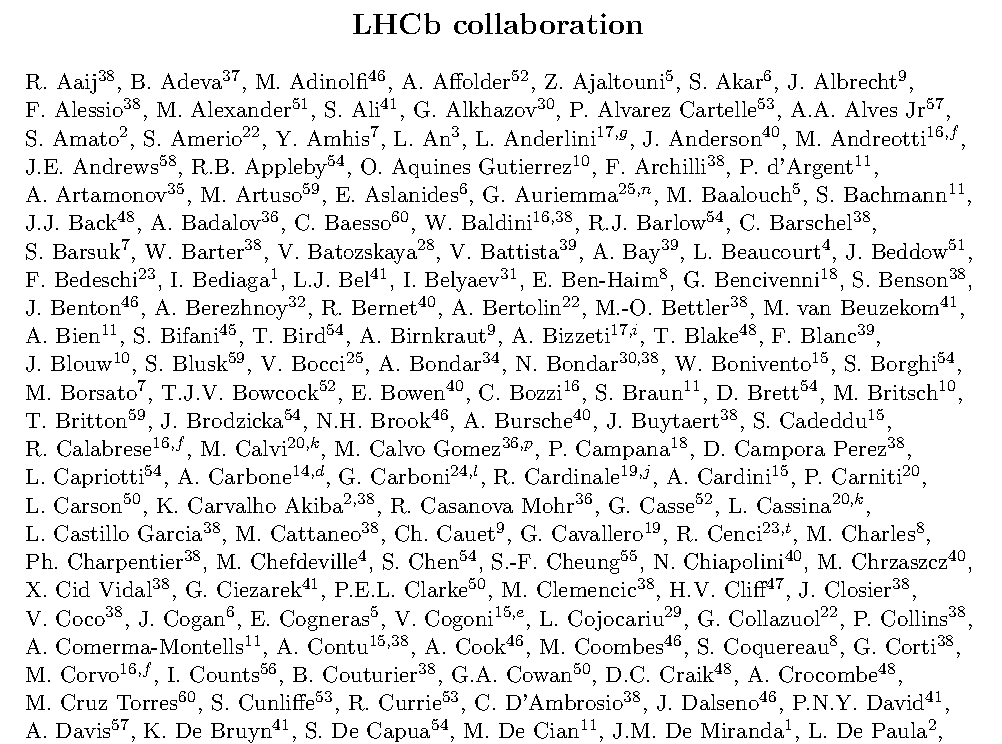
\includegraphics[width=0.45\textwidth]{Figures/authors.pdf}} & 
\subfloat[Body (normal)]{
\includegraphics[width=0.45\textwidth]{Figures/affiliations.pdf}}\\
\end{tabular}
\caption{Character class breakdown of sample lines from different sections of a CERN LHCb collaboration paper. The paper in question is the current world record holder for number of authors, and lists over 5000 authors and their affilations. The radar plots give a different impression for each of the samples.}
\end{figure}

\subsection{HEP dataset - Segmentation}
\label{subsec:hepdatasetsegmentation}

We were therefore able to experiment with combining the two datasets of HEP papers

\section{Extensions}

\begin{enumerate}
\item Confusion matrix
\item k worst files
\item Logging reprts
\item reconnecting header with segmentation model
\end{enumerate}

[INCLUDE SOME CODE HERE]

\section{Pipeline}

Python wrappers for GROBID, k fold cross validation, drawing on python libraries scikit-learn, numpy, matplotlib (pylab) etc.

[INCLUDE SOME CODE HERE]

\section{Feature Engineering}

Here we list the ideas for feature functions that we implemented and cross-validate for (see Section \ref{Chapter5}).

\subsection{Baseline}

Baseline features include token identities, prefixes, suffixes, captilisation etc.

In addition, we examined the effects of ramping up the size of the CORA set appended during training.

\subsection{Dictionaries}
\subsection{Dictionaries + Stops}
\subsection{Regularisation}

We additionally cross-validated the tuning parameter for the model, the variance for $l_2$ normalisation, $\sigma^2$, as . Unlike the true feature engineering work, this involved configuring 

\subsection{Token Extensions}

To allow this, modifications were made to GROBID to allow analysis over the full line.

\subsection{Block Shape}

\subsection{Levenshtein Distance}

\begin{equation}
  \text{lev}_{a, b}(i, j) = 
  \begin{cases} 
  	\text{max}(i, j) &\quad\text{if min(i, j) = 0} \\
	\text{min}
		\begin{cases}
			\text{lev}_{a, b}(i - 1, j) + 1 \\
			\text{lev}_{a, b}(i, j - 1) + 1 \\
			\text{lev}_{a, b}(i - 1, j - 1) + 1_{a_i \neq b_j} \\
		\end{cases} &\quad\text{otherwise} \\
  \end{cases}
\label{eq:levenshtein}
\end{equation}

\begin{equation}
\text{similarity}_{a, b} = 1 - \frac{\text{lev}_{a, b}(|a|, |b|)}{\text{max}(|a|, |b|)}
\label{eq:levenshteinsimilarity}
\end{equation}

\subsection{Character Classes}

A visual scan of any scientific paper allows one to see that lines from different sections are most easily distinguished by the composition of characters. It therefore stands to reason that we can build informative features for the \emph{segmentation} model on this basis. Thus, we see how a line may be more effectively characterised at the \emph{character} level than the \emph{word} level.

Note that the baseline feature function set does include some basic capitalisation and punctuation indicators, but we advocate our approach for several reasons:

\begin{enumerate}
\item it is more complete in that it models more character classes;
\item it does this systematically in a feature framework that is easily modified or extended, and;
\item it performs better (see Chapter \ref{Chapter5}).
\end{enumerate}

\begin{table}[h]
\begin{center}
\begin{tabular}{|c|l|l|}
\hline
Index & Class & Regex\\
\hline
0 & Spacing & \verb|r`[\s]'|\\
1 & Lower case & \verb|r`[a-z]'|\\
2 & Upper case & \verb|r`[A-Z]'|\\
3 & Numeric & \verb|r`[\d]'|\\
4 & Punctuation & \verb|r`[\(\).,?:;]'|\\
5 & Special character & \verb|r`[^\sa-zA-Z\d\(\).,?:;]'|\\
\hline
\end{tabular}
\caption[Character classes used as features, along with the regular expressions used to count them.]{Character classes used as features, along with the regular expressions used to count them.}
\label{table:characterclasses}
\end{center}
\end{table}

\begin{figure}
\centering
\begin{tabular}{cc}
\subfloat[Body (formula)]{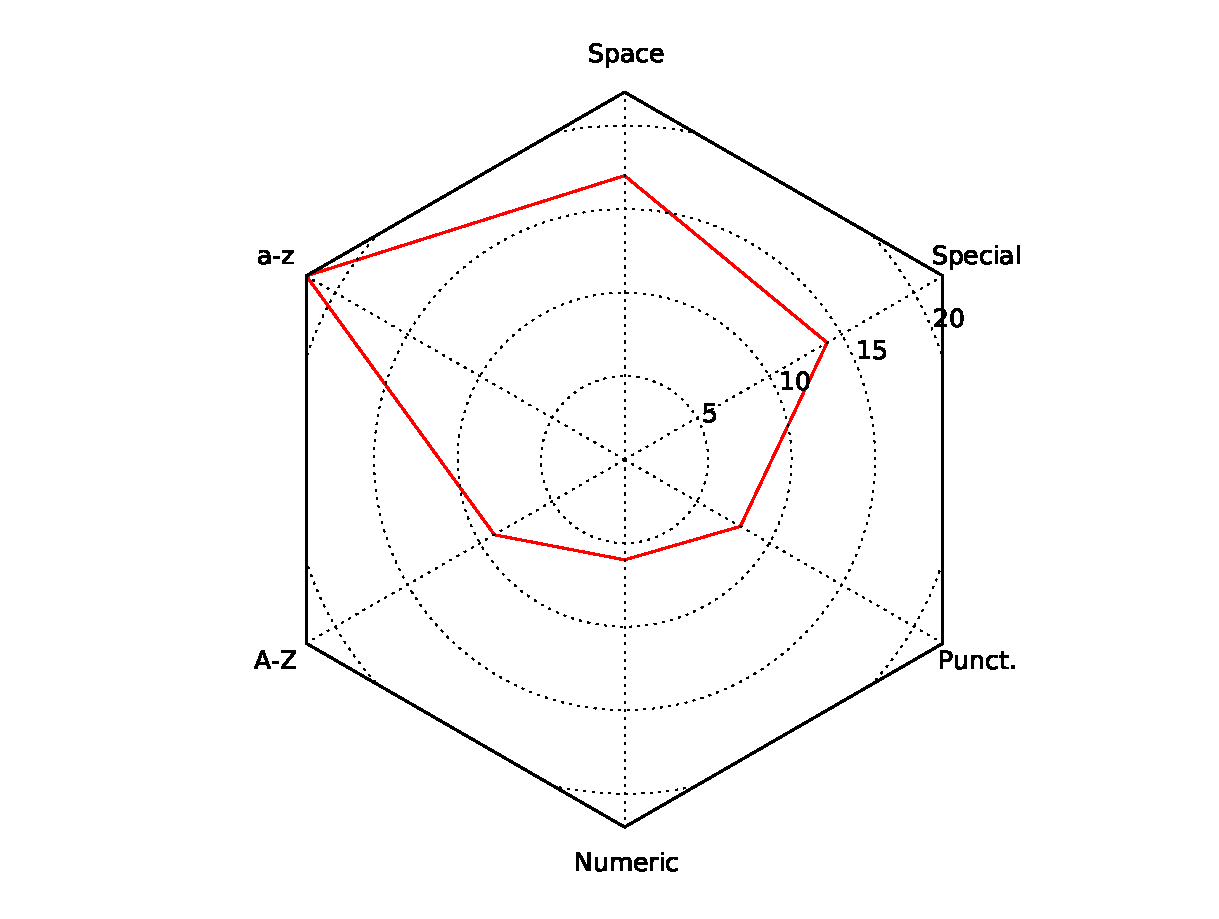
\includegraphics[width=0.5\textwidth]{Figures/body_formula.pdf}} & 
\subfloat[Body (normal)]{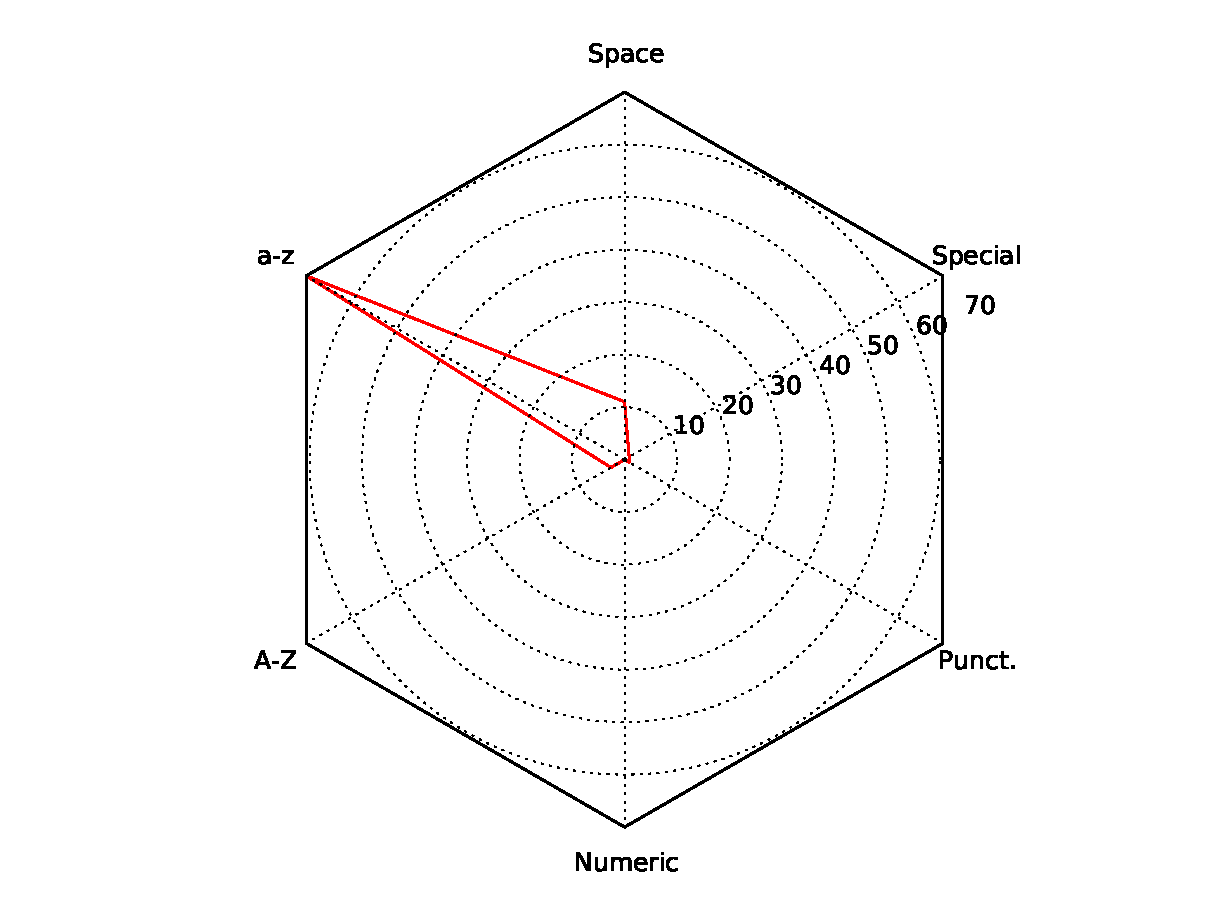
\includegraphics[width=0.5\textwidth]{Figures/body_normal.pdf}}\\
\subfloat[Headnote]{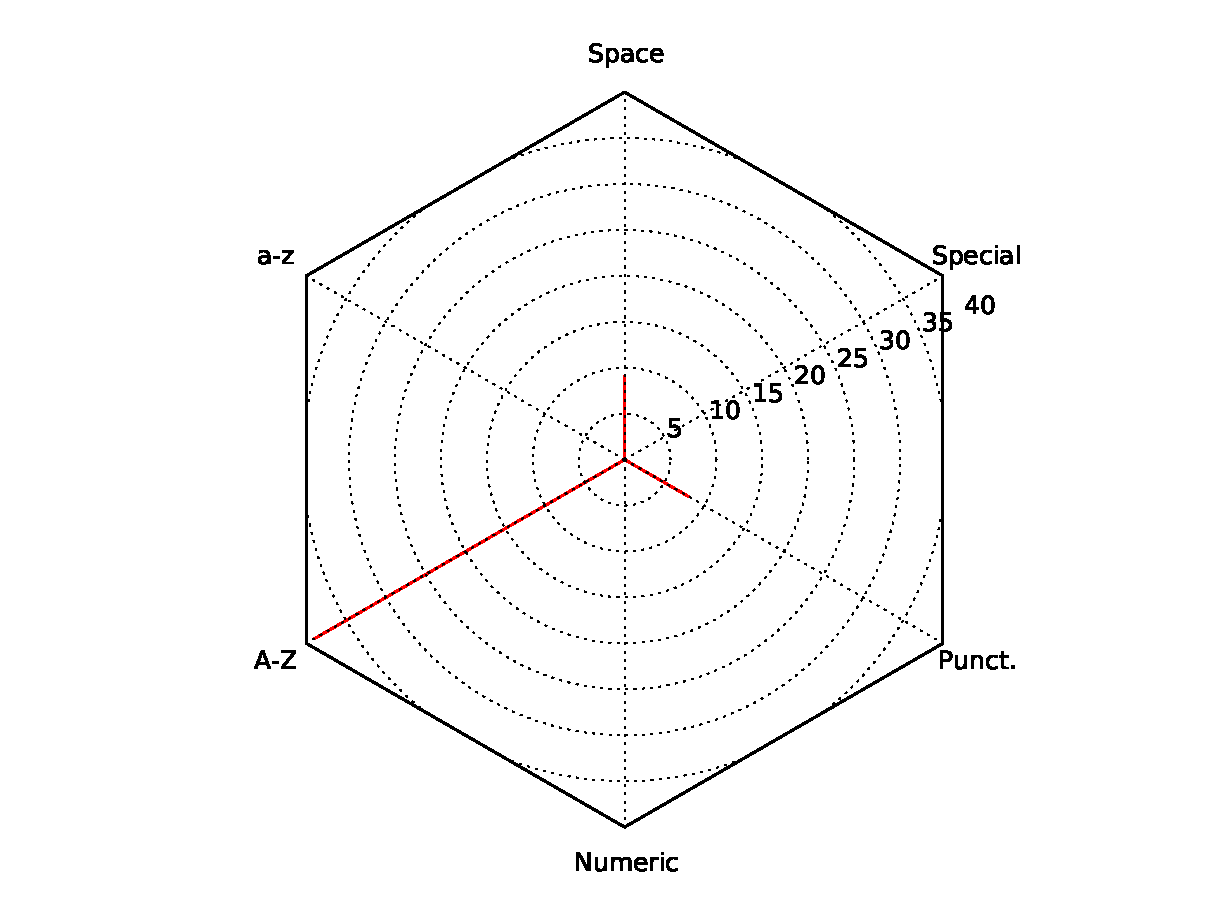
\includegraphics[width=0.5\textwidth]{Figures/headnote.pdf}}&
\subfloat[Page number]{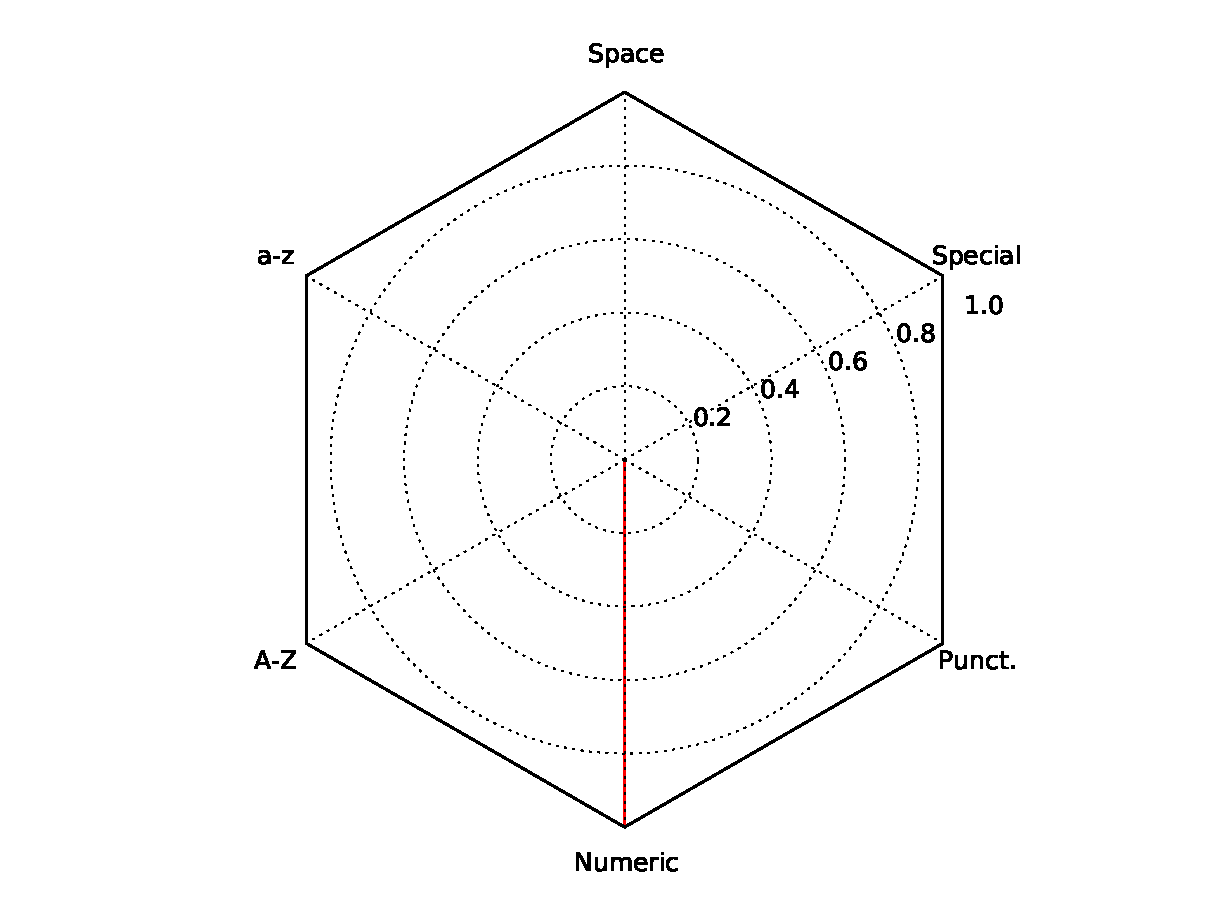
\includegraphics[width=0.5\textwidth]{Figures/page.pdf}} \\
\subfloat[Affilation list]{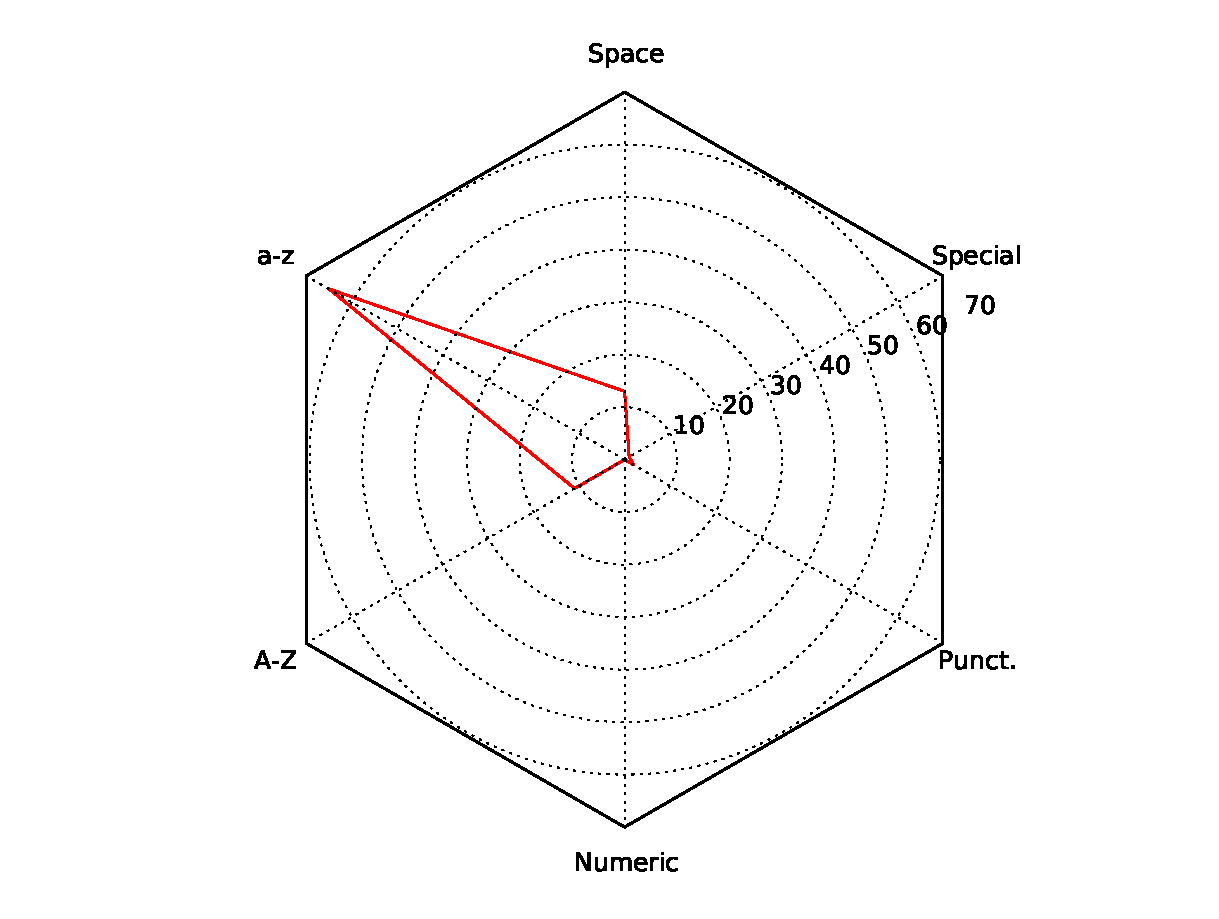
\includegraphics[width=0.5\textwidth]{Figures/affiliations_list.pdf}} & 
\subfloat[Author list]{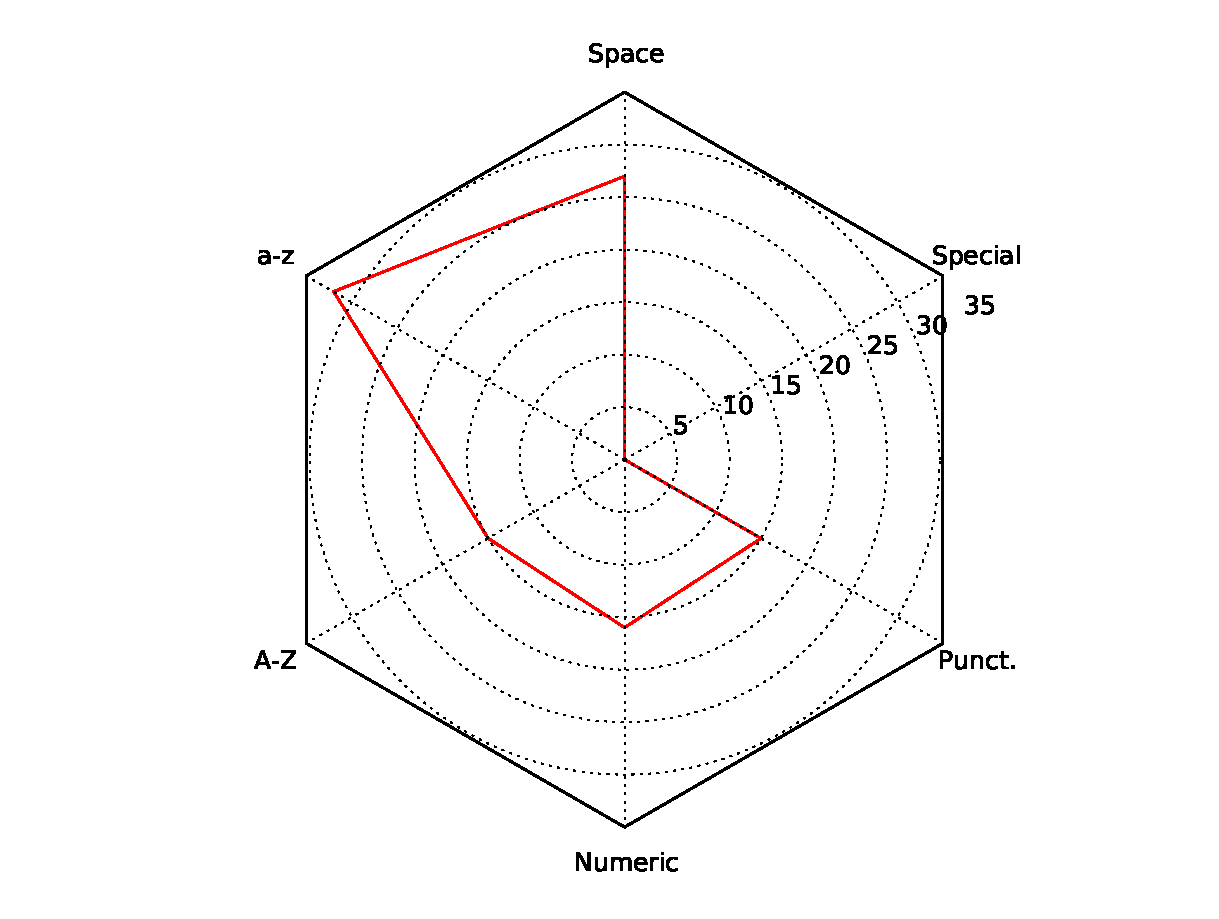
\includegraphics[width=0.5\textwidth]{Figures/author_list.pdf}} \\ 
\end{tabular}
\caption{Character class breakdown of sample lines from different sections of a CERN LHCb collaboration paper. The paper in question is the current world record holder for number of authors, and lists over 5000 authors and their affilations. The radar plots give a different impression for each of the samples.}
\end{figure}
 
% Chapter 1

\chapter{Results and Analysis} % Main chapter title

\label{Chapter5} % For referencing the chapter elsewhere, use \ref{Chapter1} 

\lhead{Chapter 5. \emph{Results and Analysis}} % This is for the header on each page - perhaps a shortened title

\emph{In this chapter we present the results of our implementation work, which comprises of 66 cross-validated feature engineering experiments including a baseline evaluation. We notably begin with a comparison between GROBID and refextract, the existing partial solution for metadata extraction within INSPIRE-HEP. Following this we detail our evaluation method and approach to running experiments. Finally, we present our experimental results and provide our analysis and interpretations.}

\section{Evaluation Method}
\subsection{Evaluation Metrics}
\label{subsec:evaluationmethod}

In this chapter we refer to various standard measures of classification performance. We define these presently. Accuracy is defined to be,

\begin{equation}
\text{Accuracy} = \frac{TP + TN}{TP + FN + FP + TN},
\label{eq:accuracy}
\end{equation}

that is, the proportion of correct classifications to total classifications, where TP is the number \emph{true positives}, the correctly predicted positive classes, where in the general case \emph{positive} refers to the given class for which we are computing accuracy; TN is the number of \emph{true negatives}, the correctly predicted \emph{negative} classes; FN is the number of \emph{false negatives}, the incorrectly predicted positive classes; and TN is the number of \emph{true negatives}. Accuracy can be a misleading statistic when we have uneven representations of classes in the dataset. In the event that we have a sufficiently high bias, we can achieve excellent accuracy simply by always predicting this class. For this reason, we consider other statistics too. \emph{Precision} is the number of times a class is \emph{correctly} predicted proportional to the overall number of times it is predicted, that is,

\begin{equation}
\text{Precision} = \frac{TP}{TP + FP}.
\label{eq:precision}
\end{equation}

This, however, does not inform us as to whether we have missed any occurences, which would be shown in the number of false negatives, FN. We could therefore have a very high precision with limited accuracy. \emph{Recall} is the number of times a class is \emph{correctly} predicted proportional to the number of occurences of that class (equivalently, the accuracy respective to the class), that is,

\begin{equation}
\text{Recall} = \frac{TP}{TP + FN}.
\label{eq:recall}
\end{equation}

However, a simple strategy of always predicting one class will give perfect recall for that class, because then misclassifications are only captured by $FP$. The $F_1$ statistic is a common measure used to assess classifiers that combines precision and recall, and is defined as,

\begin{equation}
F_1 = \frac{2 \times \text{precision} \times \text{recall}}{\text{precision} + \text{recall}},
\label{eq:f1}
\end{equation}

that is, the harmonic mean of precision and recall (the ``1'' in $F_1$ indicates the two are evenly weighted). The $F_1$ statistic is a nice way of summarising both at once as it is simply the harmonic mean of the two. Furthermore, because of this, a large imbalance in recall and precision resuts in a lower $F_1$ score. It is necessary to be good in both precision and recall to have a good $F_1$ score; the harmonic mean of any data is always upper-bounded by its arithmetic mean. Thus, the $F_1$ score addresses their shortcomings simultaneously. To summarise each of these statistics over an array of classes, we adopt two approaches: macro and micro averages. A macro average is the aggregation of statistics \emph{a posteriori}. For example, for accuracy,

\begin{equation}
\text{Accuracy}_{macro} = \frac{1}{N}\sum_{i=1}^{N}Accuracy_i,
\label{eq:macroaccuracy}
\end{equation}

where $Accuracy_i$ is the accuracy for the $ith$ of $N$ classes. By contrast, a micro average is an aggregation of statistics that is in effect weighted by population size. For example, again for accuracy,

\begin{equation}
\text{Accuracy}_{micro} = \frac{\sum_{i=1}^N TP_i + TN_i}{\sum_{i=1}^N TP_i + FN_i + FP_i + TN_i},
\label{eq:microaccuracy}
\end{equation}

\subsection{Evaluation in GROBID}

In GROBID, evaluation is done at the token, field, and instance levels, that is, GROBID calculates the aforementioned statistics for individual tokens or words, and then for the classes themselves. Finally, GROBID calculates the number of correct instances, that is, entire evaluation samples with no classification errors. In our results (Section \ref{sec:results}), we concentrate on the $F_1$ score micro average and scores for key classes (depending on the model we consider). We supplement the GROBID evaluation output with our own confusion matrices, and example of which is shown in Figure XX. Whereas the statistics allow us to compare one model to another, a confusion matrix can be used to see exactly which misclassifications are being made, which can in turn inform our feature engineering.

\section{Comparison with \emph{refextract}}

As a first result for GROBID, we compare it with \emph{refextract}, the existing solution for automatic reference extraction at CERN. \emph{refextract} is an example of a \emph{stylistic analysis} tool (see Section \ref{sec:solutionmethods}), as it employs regular expressions in a heuristic framework for metadata extraction. As previously mentioned, \emph{refextract} is incomplete and greatly lacking in both breadth and depth of detail. It is capable only of retrieving references\footnote{A comparatively easy task; GROBID's citation model usually performs at a significantly higher accuracy than, say, its \emph{header} model.}, and the classification itself is quite basic. Since the modelling of reference fields differs between the two, a comparison is difficult to make. Our results will at least be indicative, however, and we are able to make reasonable comparisons across the most important fields. The dataset for the comparison consists of 60 articles coming from the SCOAP$^3$ online repository\footnote{Scoap$^3$ (Sponsoring Open Consortium for Open Access Publishing in Particle Physics) is an open access digital library hosted at CERN, backed by an international partnership of research institutions.}.

Unlike \emph{refextract}, GROBID requires two separate models to classify the citations of a given article: the \emph{reference-segmenter} and \emph{citation} models\footnote{Strictly speaking, there is another model, (full) \emph{segmentation}, above the \emph{reference-segmenter}, and so \emph{citation} accuracy depends on this also. But because one focus of our work is to improve this model, we permit this omission.}. The \emph{reference-segmenter} model is the simplest model in GROBID's arsenal, and is responsible for segmenting a reference list block into individual references. Therefore, the accuracy of the citation model is ultimately subject to the accuracy of the reference block inputs supplied to it by the \emph{reference-segmenter} above. The results for training and evaluating the \emph{reference-segmenter} on 60 SCOAP$^3$ papers with an 80--20 split are given in Table \ref{table:referencesegmenterresults}. The results show the \emph{reference-segmenter} is extremely accurate. In fact, only 5 token misclassifications out of 622 were made for the <label> class, and from a grand total of 12,981.

\label{subsec:refextract}
\begin{table}[h]
\begin{center}
\begin{tabular}{|c|cccc|}
\hline
label           & accuracy  & precision  & recall   & f1 \\
\hline
<label>         & 99.96     & 100        & 99.2     & 99.6\\
<reference>     & 99.96     & 99.96      & 100      & 99.98\\
\hline
(micro average) & 99.96     & 99.96      & 99.96    & 99.96  \\
(macro average) & 99.96     & 99.98      & 99.6     & 99.79  \\
\hline
\end{tabular}
\caption[Token-level evaluation results for reference segmentation.]{Token-level evaluation results for reference segmentation.}
\label{table:referencesegmenterresults}
\end{center}
\end{table}

The most significant difference between the tools is the set of classes modelled. \emph{refextract} attempts only to classify to the minimum detail required for identifying the originating document within INSPIRE-HEP. Therefore, there are no equivalents to GROBID's classes, <volume>, <pages>, and so on. Rather, these parts of references are absorbed into other, higher-level classes, and are indicated by a dash (-) in the results table, Table \ref{table:citationcomparison}. Comparisons can be made, however on fields, <title>, <author>, <journal>, and <date>. There we see the superiority of GROBID over \emph{refextract}. Note that here the \emph{citation} model was not trained on the evaluation set, and in particular this may explain its dismal performance in precision for the date field, and recall for \emph{pubnum}. The dataset instances contained a recurring publication number that was almost uniformly misclassified by GROBID as a date. Notice that this is an example of a domain specificity of HEP papers. Had we trained on these papers, we could expect an improvement. That \emph{refextract} has reported perfect recall is a result of a flaw in our simplistic evaluation, where missing expected classifications were simply assigned to a \emph{null} class, and so \emph{false positives} (FP) were not counted; only \emph{false negatives}. Therefore, the true performance of \emph{refextract} is upper-bounded by the figures in Table \ref{table:citationcomparison}. The table is one of the outputs of GROBID's evaluation utilities. For an explanation of the performance metrics, see Section \ref{subsec:evaluationmethod}.

\begin{table}[h]
\begin{center}
\begin{tabular}{|c|cccc|cccc|}
\hline
engine &  \multicolumn{4}{c|}{GROBID} & \multicolumn{4}{c|}{\emph{refextract}}\\
\hline
label & accuracy & precision & recall & f1 & acc. & prec. & rec. & f1\\
\hline
<author>    & 99.85 &   99.68   &   99.75   &   99.72   & 98.33 &   100 &   92.22   &   95.95   \\
<title> &   99.59   &   98.87   &   99.25   &   99.06   & 94.89 &   100 &   71.75   &   83.55   \\
<journal>   & 98.84 &   88.87   &   93.98   &   91.35   & 97.12 &   100 &   46.78   &   63.74   \\
<volume>&   99.95   &   99.07   &   98.15   &   98.6    & -     &   -   &   -       &   -   \\
<issue> &   99.93   &   100     &   94.63   &   97.24   & -     &   -   &   -       &   -   \\
<pages> &   99.75   &   93.51   &   99.45   &   96.39   & -     &   -   &   -       &   -   \\
<date>  &   98.39   &   57.39   &   98.31   &   72.47   & 98.88 &   100 &   37.55   &   54.6    \\
<pubnum>&   98.71   &   100     &   12.96   &   22.95   & -     &   -   &   -       &   -   \\
<note>  &   99.4    &   43.75   &   35      &   38.89   & -     &   -   &   -       &   -   \\
<publisher>&99.81   &   63.46   &   94.29   &   75.86   & -     &   -   &   -       &   -   \\
<location>& 99.81   &   86.32   &   91.11   &   88.65   & -     &   -   &   -       &   -   \\
<institution>& 99.78&   25      &   25      &   25      & -     &   -   &   -       &   -   \\
<booktitle>&    98.7&   55.56   &   41.67   &   47.62   & -     &   -   &   -       &   -   \\
<web>   &   99.64   &   51.85   &   100     &   68.29   & -     &   -   &   -       &   -   \\
<editor>    &  99.93&   100     &46.67      &   63.64   & -     &   -   &   -       &   -   \\
<tech>  &   99.95   &   83.33   &   50      &   62.5    & -     &   -   &   -       &   -   \\
\hline
(micro average) & 99.5  &   93.63   &   94.77   &   94.19 & -    &   - &   -   &   -   \\
(macro average) & 99.5  &   77.92   &   73.76   &   71.76 & -    &   -  &   -   &   -   \\
\hline
\end{tabular}
\caption[Token-level evaluation results for citations for GROBID and \emph{refextract}.]{Token-level evaluation results for citations for GROBID and \emph{refextract}.}
\label{table:citationcomparison}
\end{center}
\end{table}

\section{Experiment Setup}
\label{sec:experimentsetup}

Our resources for experimentation consisted of two powerful virtual machines on the CERN LXPLUS computing cluster, each possessing 16 CPUs and 32 GB of RAM. The experiments were configured and uploaded to these server machines in batches, and were processed by our experimentation pipeline (see Section \ref{subsec:pipeline}). The sparse nature of the models led to long training times. To control the runtime of training, we enforced a maximum number of 500 iterations for Wapiti's L-BFGS algorithm. This number was chosen from observing the diminishing improvements of models trained to this extent\footnote{There is also the argument that training to convergence may cause overfitting.}. With Wapiti parallelised to 8 cores, we were able to run two processes on each virtual machine when required. Even with this parallelised setup, our experiment batches took several days to process each time, and the sum total of our experiments amounts to perhaps months of CPU time.

In conjunction with our feature engineering variations, we tried different configurations of data. Figure \ref{fig:cv} illustrates our five approaches to cross-validation with different combinations of HEP and CORA training data. Where we \emph{append} data, we include it in the training, but exclude from the evaluation. Thus, HEP app. CORA denotes the training of a model on, but cross-validation folds taken only from the HEP. Of most interest, naturally, were those evaluating purely on HEP papers, that is, those we denote \emph{HEP} and {HEP app. CORA}, and these were the only configurations run beyond the baseline. In Section \ref{sec:results}, we refer to these configurations as we present the results. All experiments were run with $5-$fold cross validation.

\begin{figure}[h]
\centering
\begin{tabular}{cc}
\subfloat[CV HEP]{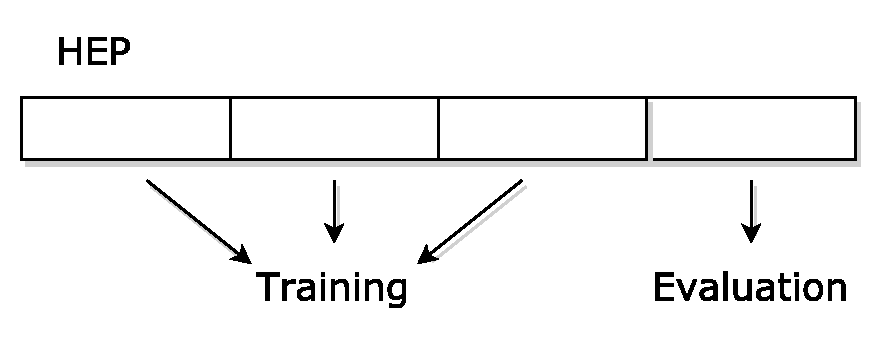
\includegraphics[width=0.36\textwidth]{Figures/CV_HEP.pdf}} & 
\subfloat[CV CORA]{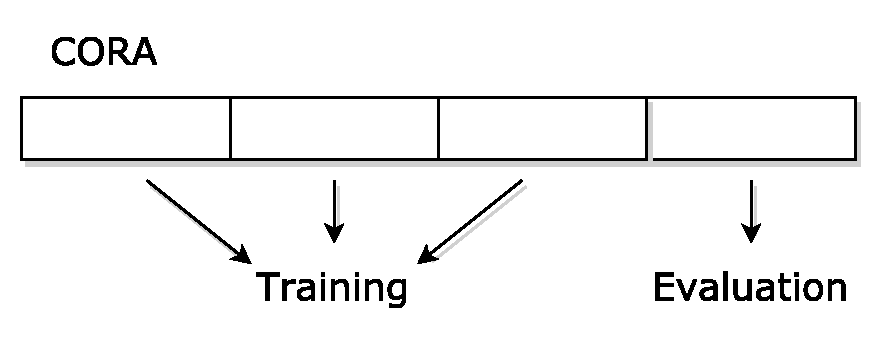
\includegraphics[width=0.36\textwidth]{Figures/CV_CORA.pdf}}\\
\subfloat[CV HEP append CORA]{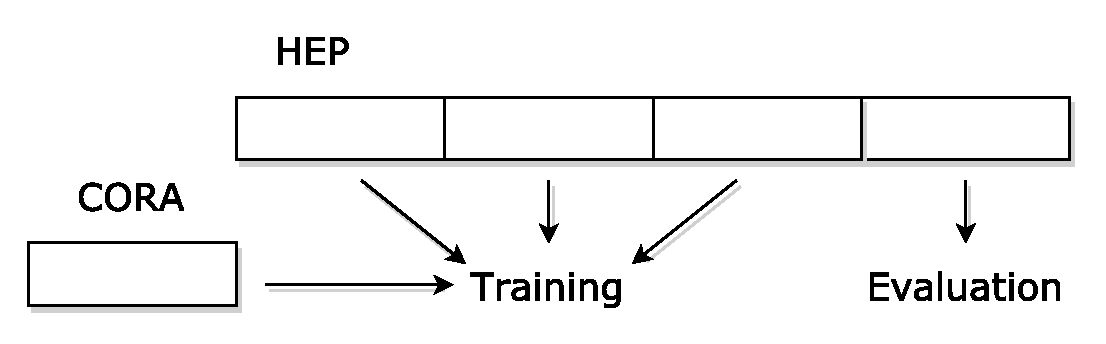
\includegraphics[width=0.45\textwidth]{Figures/CV_HEPappCORA.pdf}} & 
\subfloat[CV CORA append HEP]{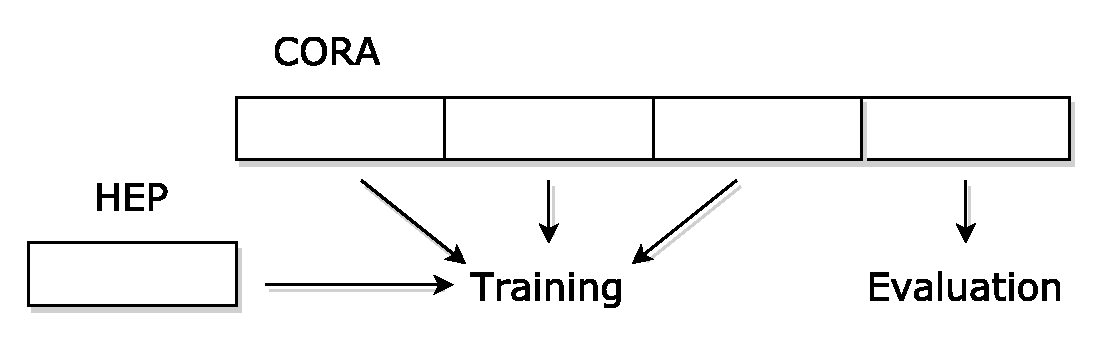
\includegraphics[width=0.45\textwidth]{Figures/CV_CORAappHEP.pdf}}\\ 
\multicolumn{2}{c}{\subfloat[CV HEP + CORA]{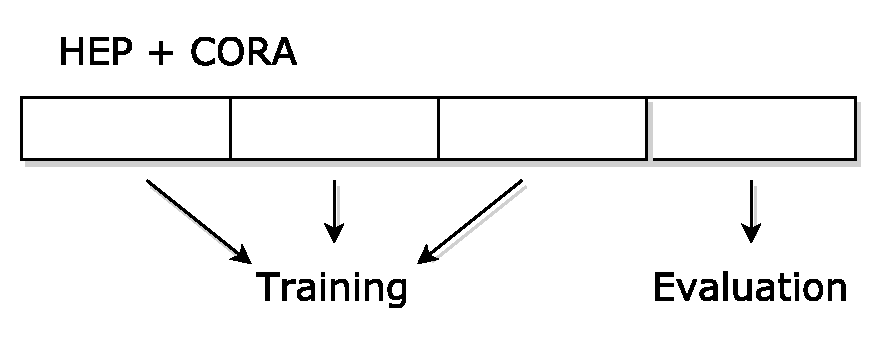
\includegraphics[width=0.36\textwidth]{Figures/CV_HEP+CORA.pdf}}} \\
\end{tabular}
\caption{The different cross-validation configurations used in our experiments. Figures (A) and (B) show cross-validation on HEP and CORA sets independently, and (E) on their combination. Figures (C) and (D) show cross-validation on the HEP and CORA datasets respectively, appending the other at training time.}
\label{fig:cv}
\end{figure}

The variety of $66$ experiments that we cross-validated are presented in Table \ref{fig:cv}, organised into 8 categories. We also distinguish by model, running some experiments for both models, and some for one alone. Generally speaking, we chose feature engineering ideas with a particular model in mind, that is, either \emph{header} or \emph{segmentation}. Finally, we distinguish by the data configurations. For dictionary-based features, whcih may be derived from a baseline feature file alone, we may try all data configurations. However, as we do not have access to the original PDF papers for the CORA dataset, we cannot extract our new features. In these cases, our cross-validation was performed on our own purely HEP dataset.


\begin{table}[h]
\begin{center}
\begin{tabular}{ | p{0.2\linewidth} | p{0.25\linewidth} | p{0.15\linewidth} | p{0.3\linewidth} |}
\hline
Feature Category & Variations & Models & Data\\
\hline
Baseline & - & Segmentation, header & CORA, CORA app. HEP, CORA + HEP, HEP, HEP app. CORA \\
\hline
Baseline & - & Header & HEP app. 1/3 CORA, HEP app. 2/3 CORA \\
\hline
Dictionaries & First order, second order, third order & Segmentation, header & HEP, HEP app. CORA \\
\hline
Dicts. + Stops & First order, second order, third order, stops only & Segmentation, header & HEP, HEP app. CORA \\
\hline
Regularisation & $\sigma^2=0$, $\sigma^2=\exp\{-6\}$, $\sigma^2=\exp\{-5\}$, $\sigma^2=\exp\{-4\}$, $\sigma^2=\exp\{-3\}$, & Header & HEP \\
\hline
Token Extension & First 5 words, first 10, first 15, first 20 & Segmentation & HEP \\
\hline
Block Size & Height, width, height \& width, area & Header & HEP \\
\hline
Levenshtein & $T_1 = 0.05$, $T_1 = 0.1$, $T_1 = 0.2$, $T_1 = 0.4$, $T_1 = 0.8$, ($T_1 = 0.1, T_2 = 0.4$), All & Segmentation & HEP \\
\hline
Character Classes & Binary, decimal (round down), decimal (round), decimal (20 point) & Segmentation & HEP \\
\hline
\end{tabular}
\caption[A summary of our experiments, organised by category, models trained for, and data configurations used.]{A summary of our experiments, organised by category, models trained for, and data configurations used.}
\label{table:experiments}
\end{center}
\end{table}

\section{Results}
\label{sec:results}
\subsection{Baseline}

We were therefore able to experiment with combining the two datasets of HEP papers, as well as subsampling the CORA dataset to find the ideal mixture. After all, in spite of the common wisdom that increasing the amount of training data will improve generalisation and model performance, it is not clear what effects combining different ground truths, namely CORA and HEP, will have. One may imagine that generalising over a hybrid dataset might construct a misleading model when it comes to evaluate on a pure HEP dataset, especially when the CORA \emph{header} set dwarfs our HEP one.

\begin{figure}[h]
\center
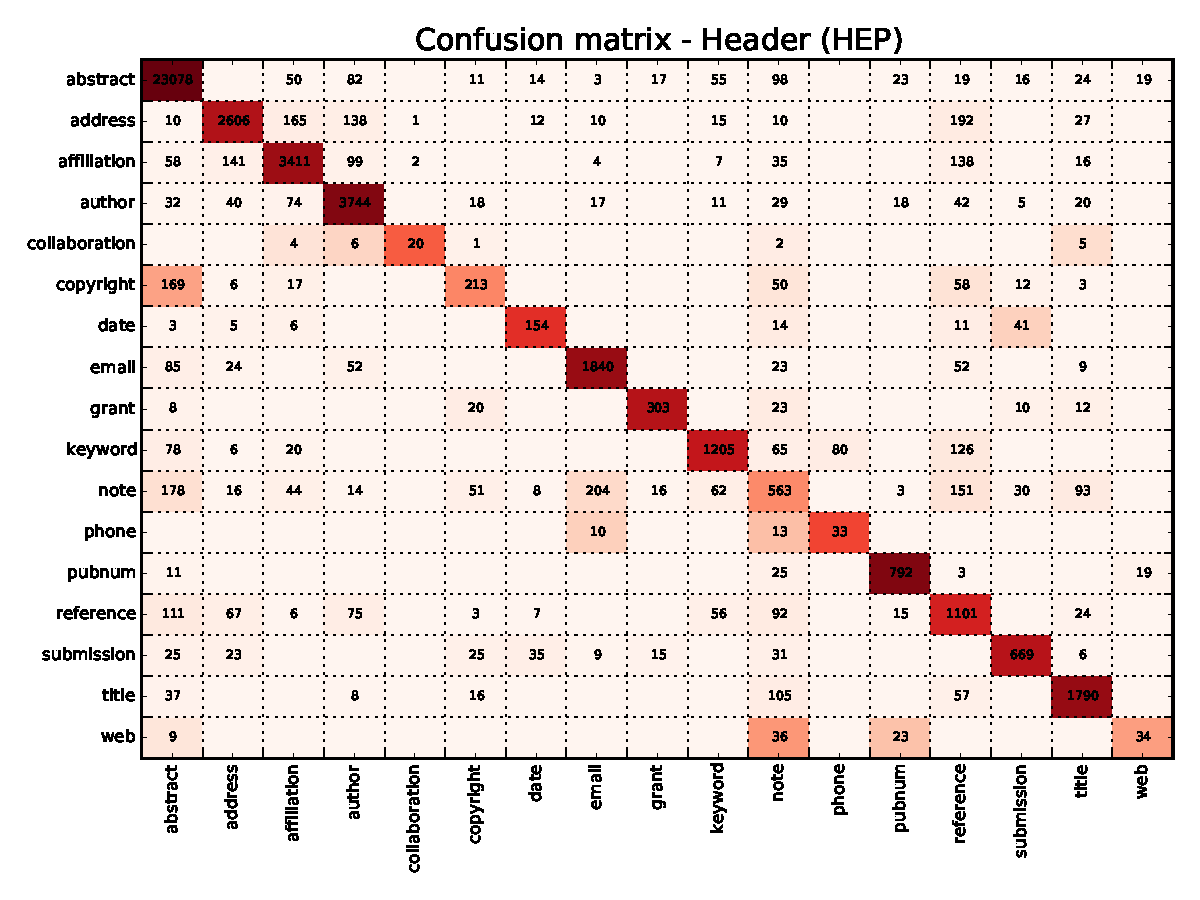
\includegraphics[width=5.5in]{Figures/header_baseline_confusion.pdf}
\caption{}
\label{fig:header_baseline_confusion}
\end{figure}

\begin{figure}[h]
\center
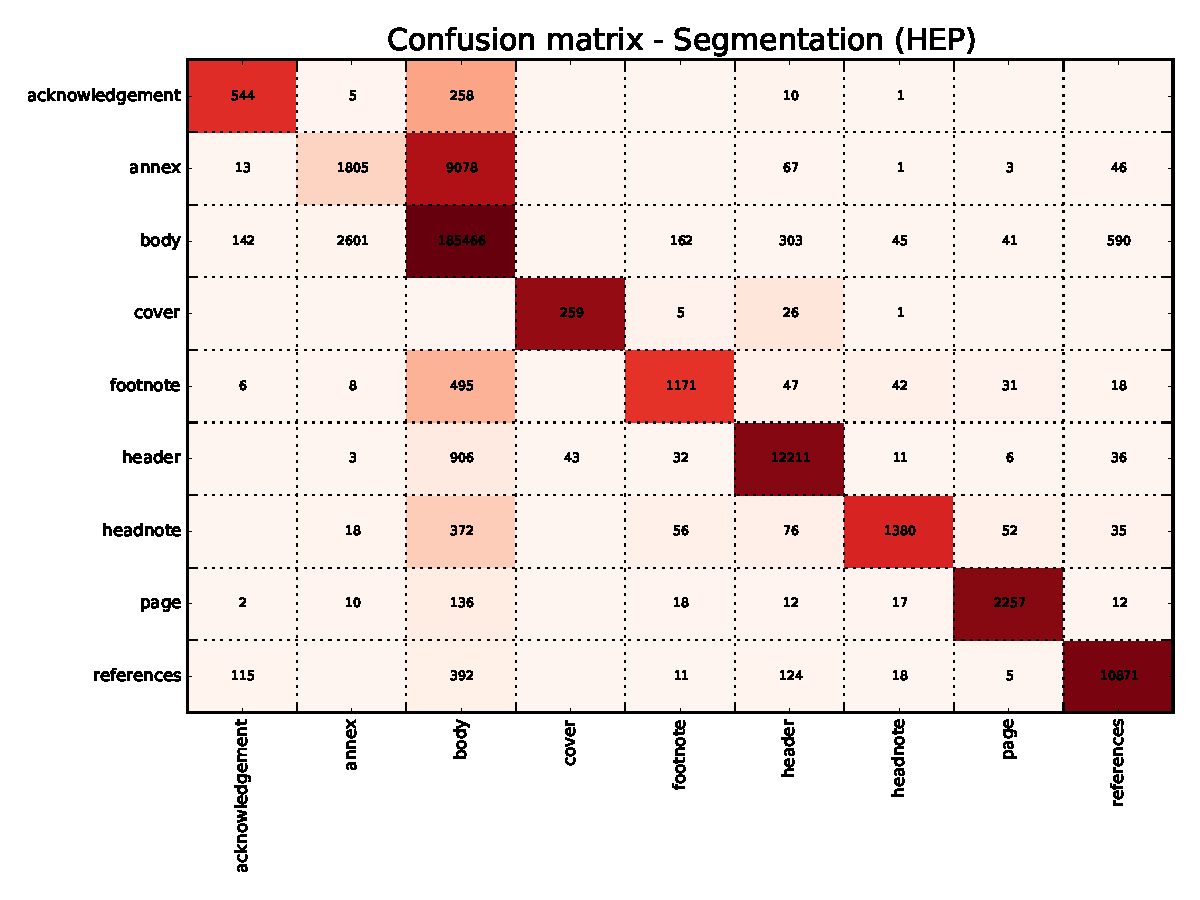
\includegraphics[width=5.5in]{Figures/segmentation_baseline_confusion.pdf}
\caption{}
\label{fig:segmentation_baseline_confusion}
\end{figure}

\begin{figure}[h]
\center
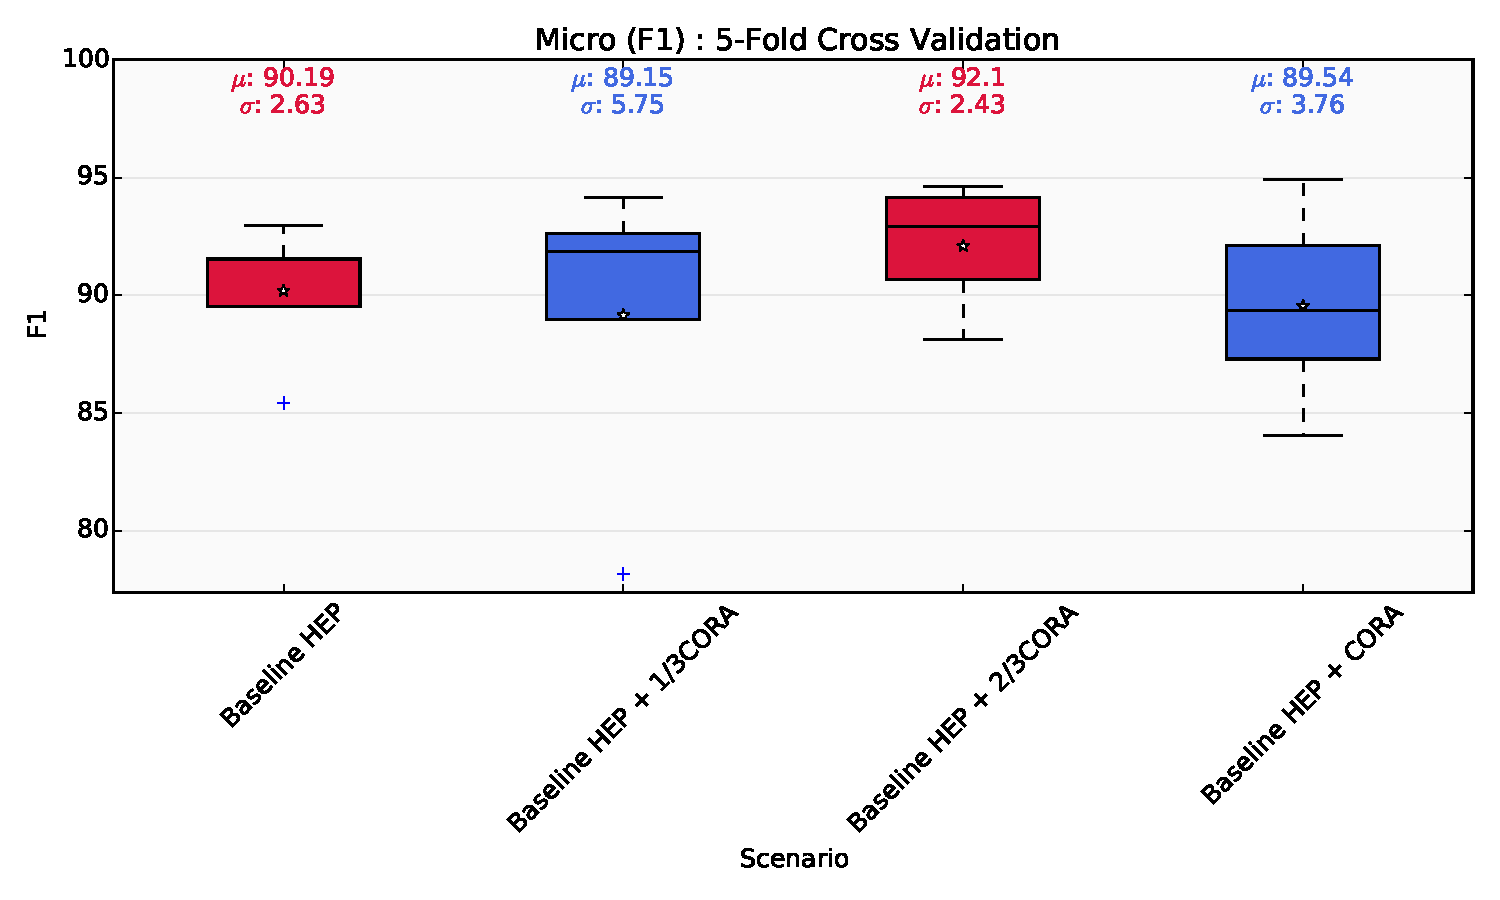
\includegraphics[width=5.5in]{Figures/micro_subsampling.pdf}
\caption{}
\label{fig:references}
\end{figure}


\subsection{Block Size}

\subsection{Character Classes}

\subsection{Dictionaries}

\subsection{Dictionaries + Stop Words}

\subsection{Levenshtein}

\subsection{Regularisation}

\subsection{Token Selection}

\subsection{Results Summary}

\begin{figure}[h]
\center
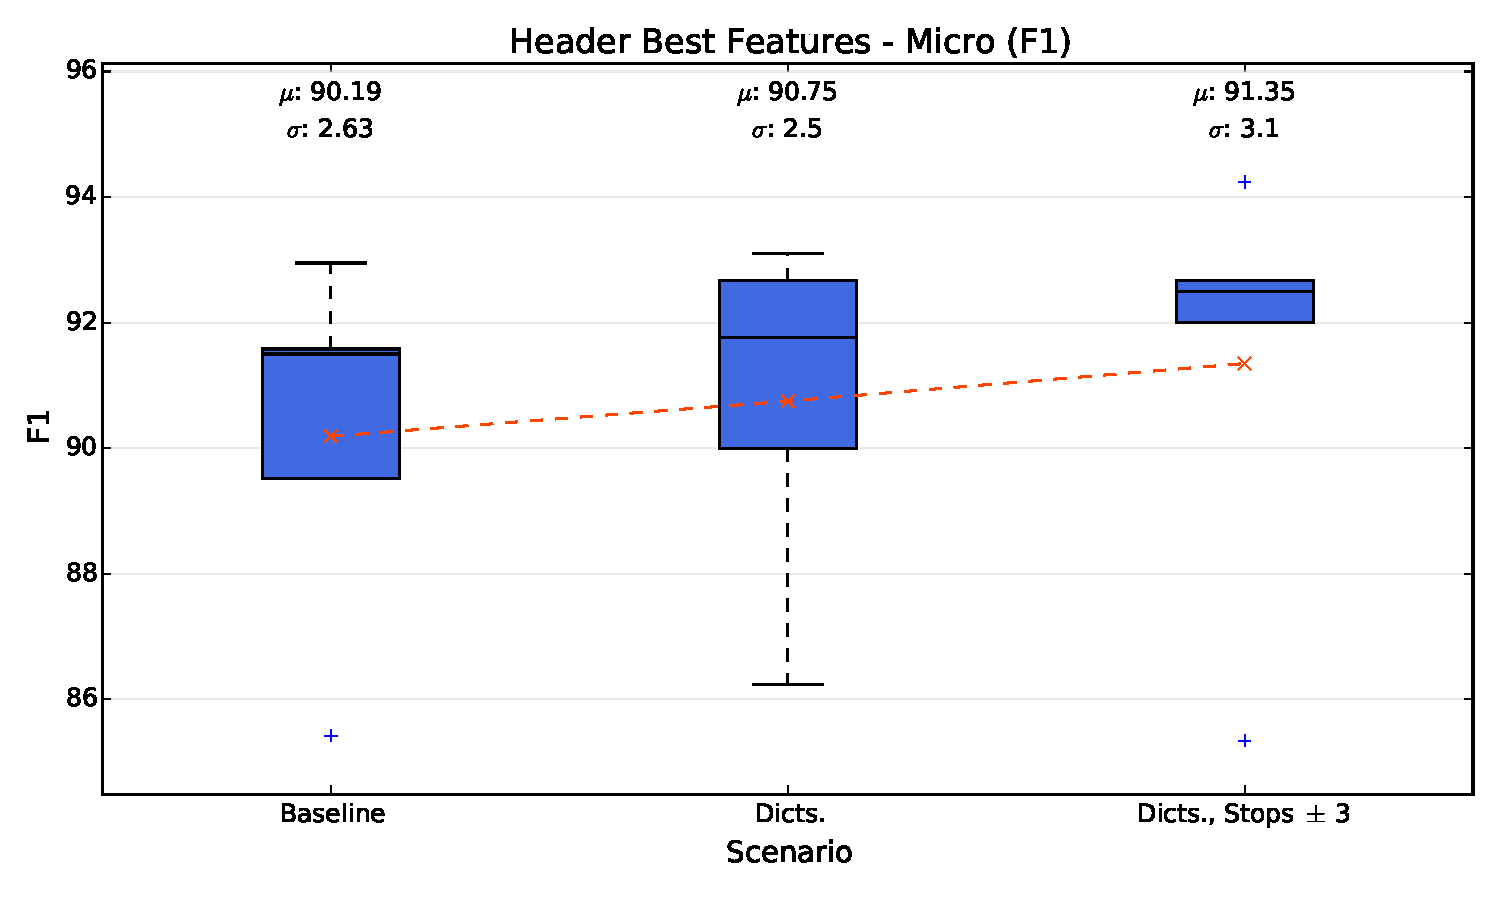
\includegraphics[width=5.5in]{Figures/micro.pdf}
\caption{}
\label{fig:micro}
\end{figure}

\begin{figure}[h]
\center
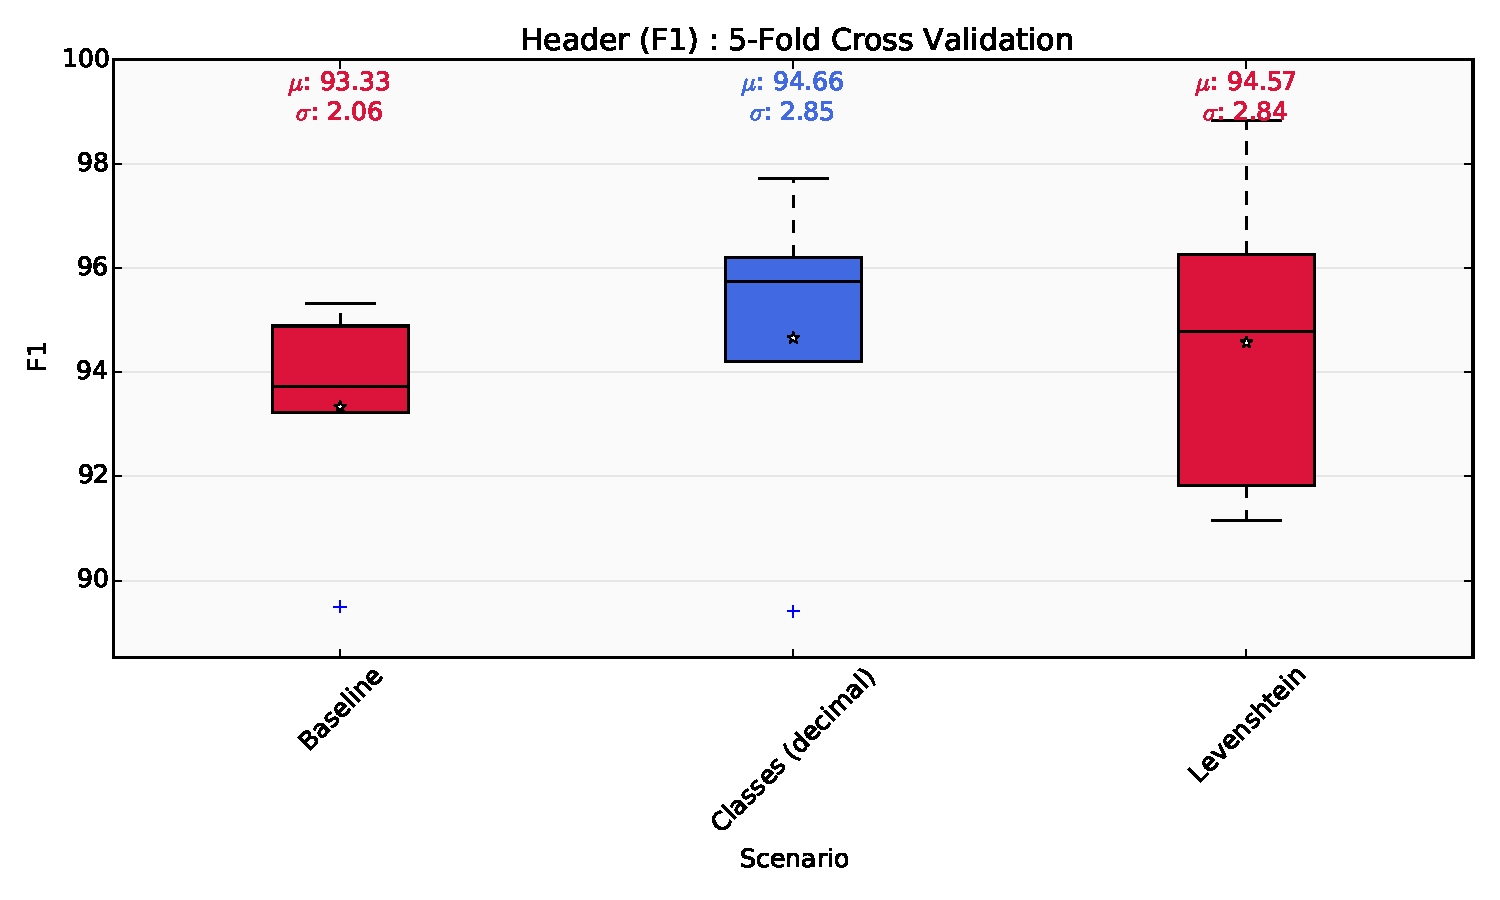
\includegraphics[width=5.5in]{Figures/header.pdf}
\caption{}
\label{fig:header}
\end{figure}

\begin{figure}[h]
\center
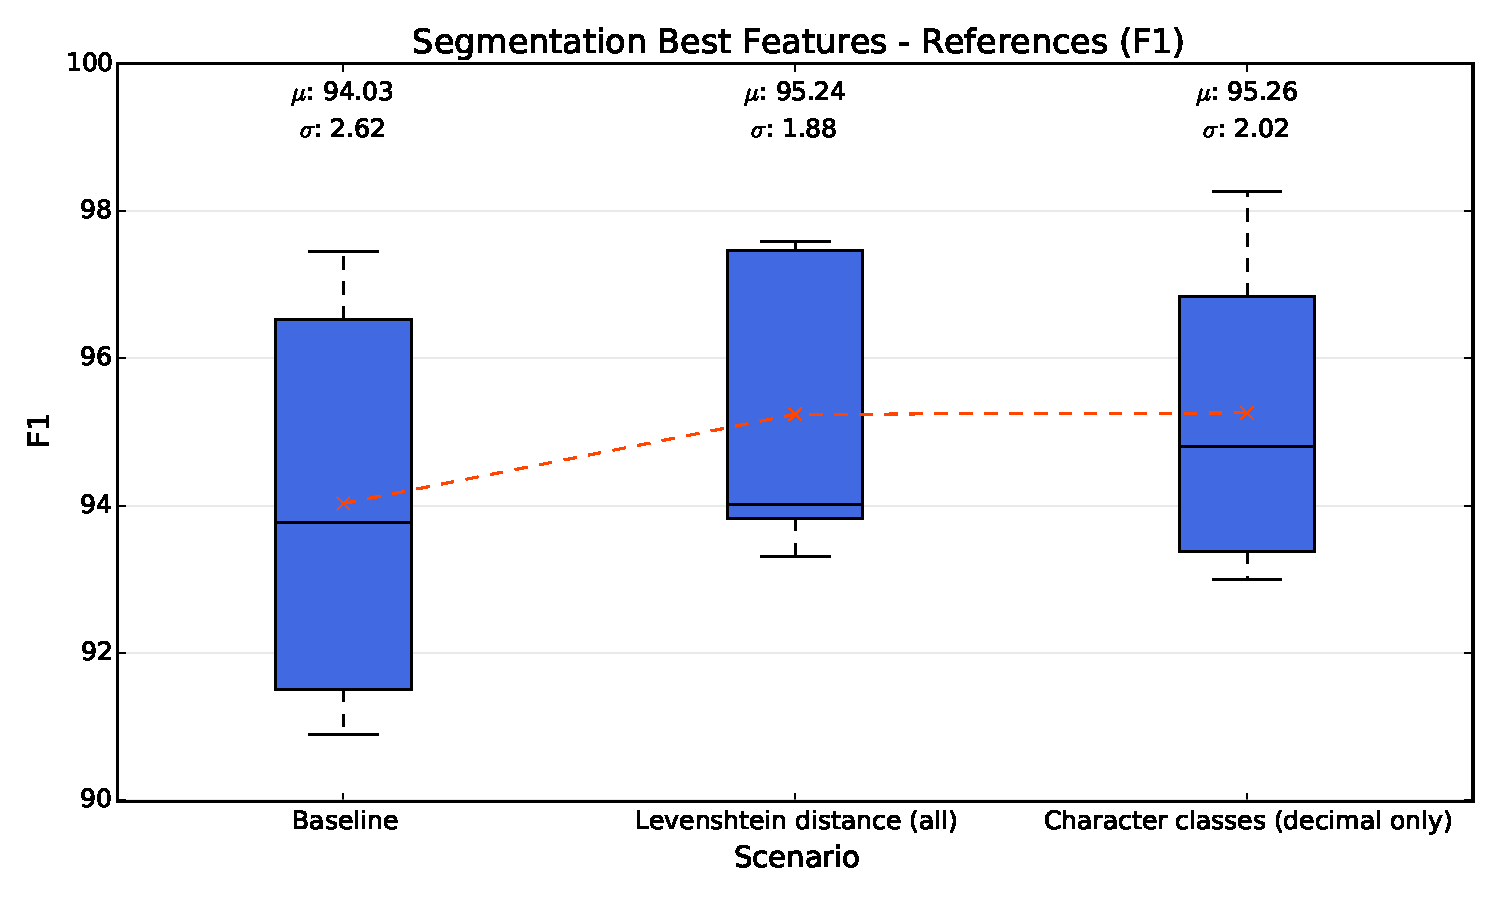
\includegraphics[width=5.5in]{Figures/references.pdf}
\caption{}
\label{fig:references}
\end{figure}
 
% Chapter 1

\chapter{Conclusion} % Main chapter title

\label{Chapter6} % For referencing the chapter elsewhere, use \ref{Chapter1} 

\lhead{Chapter 6. \emph{Conclusion}} % This is for the header on each page - perhaps a shortened title

%----------------------------------------------------------------------------------------

\section{Summary}
\subsection{Key Results}
\section{Future Work}

Different training algorithm and regularisation.
Emulating our modelling of head collaborations in references.
Expanding training set (it turns out HEP papers are distinct from )

\label{sec:futurework} 
%\input{Chapters/Chapter7} 

%----------------------------------------------------------------------------------------
%	THESIS CONTENT - APPENDICES
%----------------------------------------------------------------------------------------

\addtocontents{toc}{\vspace{2em}} % Add a gap in the Contents, for aesthetics

\appendix % Cue to tell LaTeX that the following 'chapters' are Appendices

% Include the appendices of the thesis as separate files from the Appendices folder
% Uncomment the lines as you write the Appendices

% Appendix A

\chapter{Algorithms} % Main appendix title

\label{AppendixA} % For referencing this appendix elsewhere, use \ref{AppendixA}

\lhead{Appendix A. \emph{Appendix Title Here}} % This is for the header on each page - perhaps a shortened title

\begin{algorithm}[!ht]
 \KwData{Observation sequence, $\mathbf{x}$, and model parameters, $\theta=(\mathbf{A}, \mathbf{B}, \mathbf{I})$}
 \KwResult{Most likely sequence, \textbf{y*}}
 Initialise $\mathbf{y}*$ as a zero-length sequence
  \For {s $\in$ S}{
   $v_1(s) = \mathbf{I}(s) \times \mathbf{B}(x_1, s)$
  }
  \For{$t = 2$ to T}{
   \For{s $\in$ S}{
    $v_t(s) = \max_{s'}(\mathbf{A}(s', s) \times v_{t-1}(s')) \times \mathbf{B}(x_t, s)$ \\
    Append s to $\mathbf{y}*$
    }
 }
 Return $\mathbf{y}*$
 \caption{The Viterbi algorithm ($\mathcal{O}(T|S|^2))$ for computing the most likely hidden sequence for a given observation sequence of an HMM.}
 \label{alg:viterbi}
\end{algorithm}

\begin{algorithm}[!ht]
 \KwData{Observation sequence, $\mathbf{x}$, and model parameters, $\theta=(\mathbf{A}, \mathbf{B}, \mathbf{I})$}
 \KwResult{Set of forward variables, $\{\alpha_t(s)\}_{s \in S, t \in T}$, and backward variables, $\{\beta_t(s)\}_{s \in S, t \in T}$}
 \For {$s \in S$}{
  $\alpha_1(s) = B(x_1, s) \times \mathbf{I}(s)$ \\
  \For {t = 2 to T}{
   $\alpha_t(s) = \sum_{s'} \mathbf{A}(s, s')  \times \mathbf{B}(x_t, s) \times \alpha_{t-1}(s')$
  }
 }
 \For {$s \in S$}{
  $\beta_T(s) = 1$ \\
  \For {t = T-1 to 1}{
   $\beta_t(s) = \sum_{s'} \beta_{t+1}(s') \times \mathbf{A}(s, s')  \times \mathbf{B}(x_t, s)$
  }
 }
Return the sets of backward and forward variables
\caption{The forward-backward algorithm - $\mathcal{O}(T|S|^2)$}
\label{alg:fb}
\end{algorithm}
%% Appendix B

\chapter{Figures} % Main appendix title

\label{AppendixB} % For referencing this appendix elsewhere, use \ref{AppendixA}

\lhead{Appendix B. \emph{Figures}} % This is for the header on each page - perhaps a shortened title

\begin{figure}[!ht]
\center
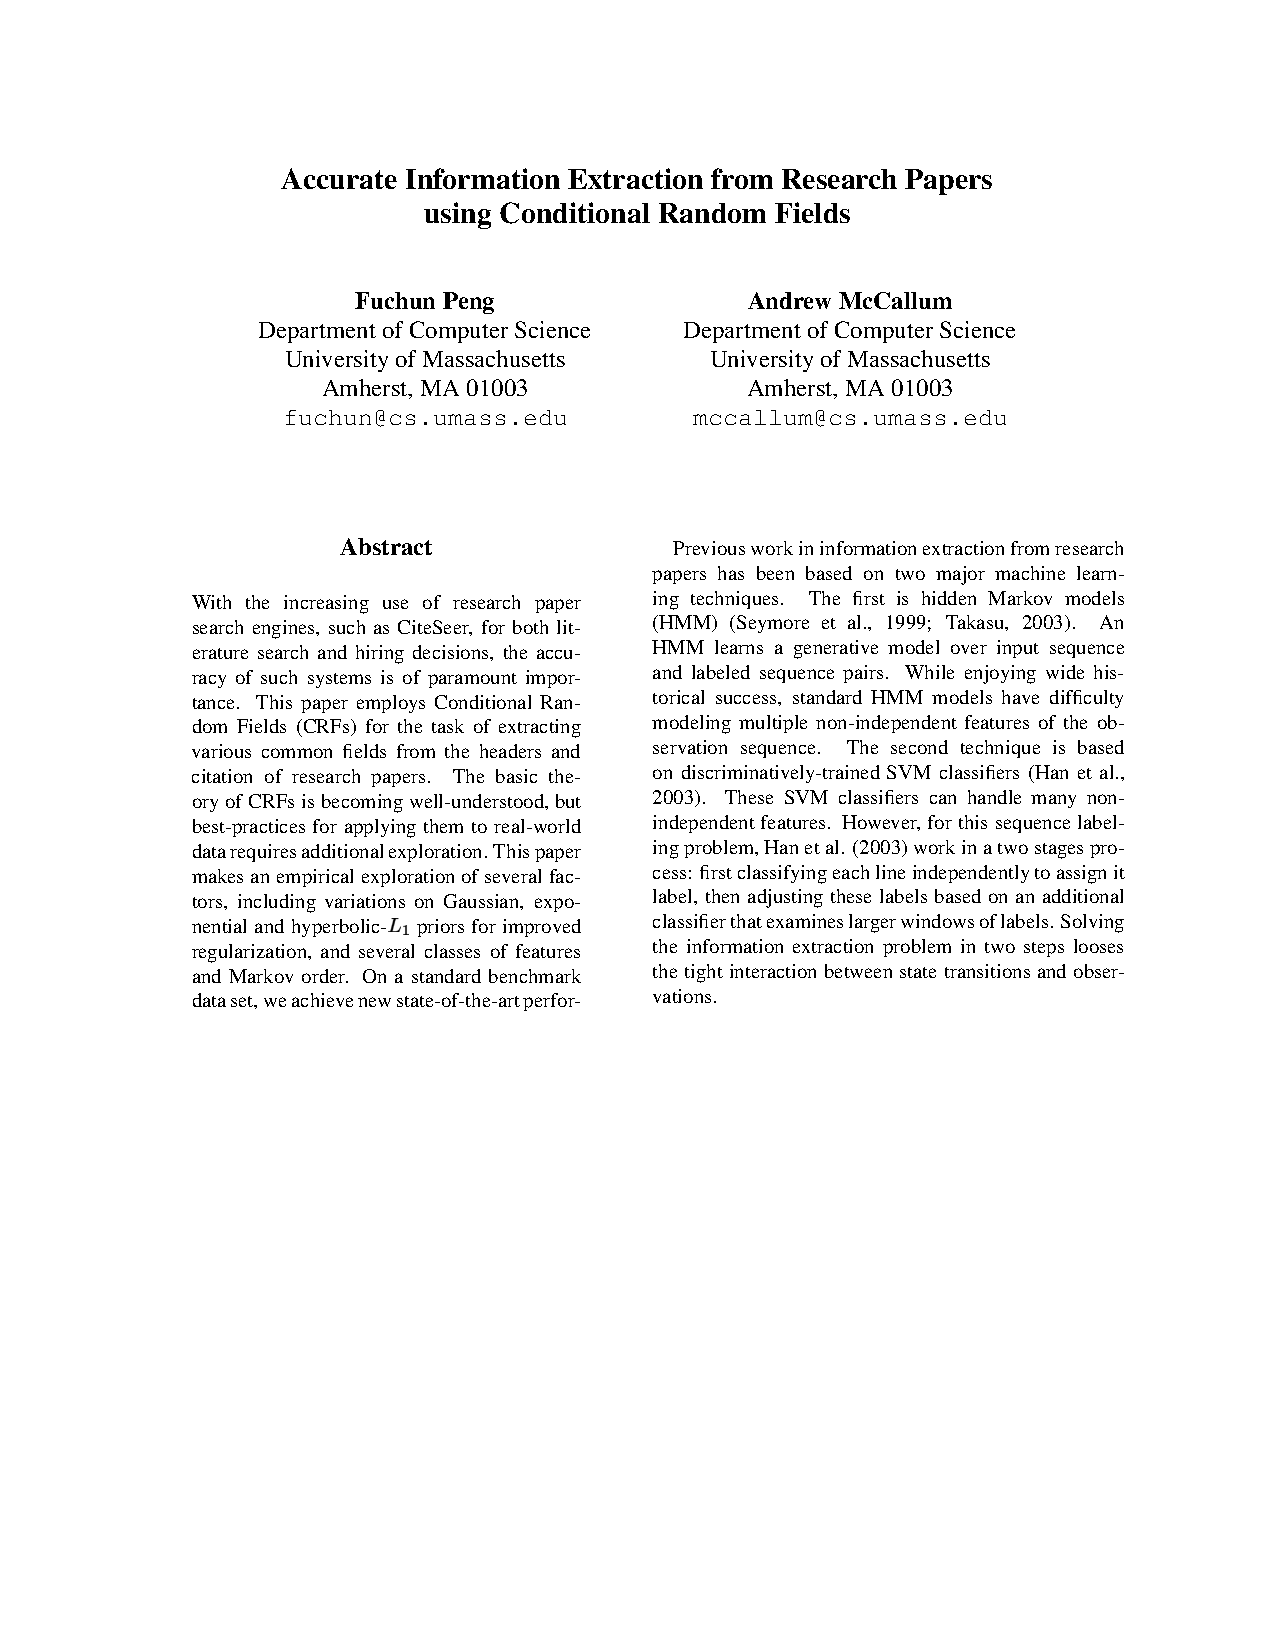
\includegraphics[width=3.25in]{Figures/header1.pdf}
\caption{The header section of a scientific paper.}
\label{fig:HMM}
\end{figure}

\begin{figure}[!ht]
\center
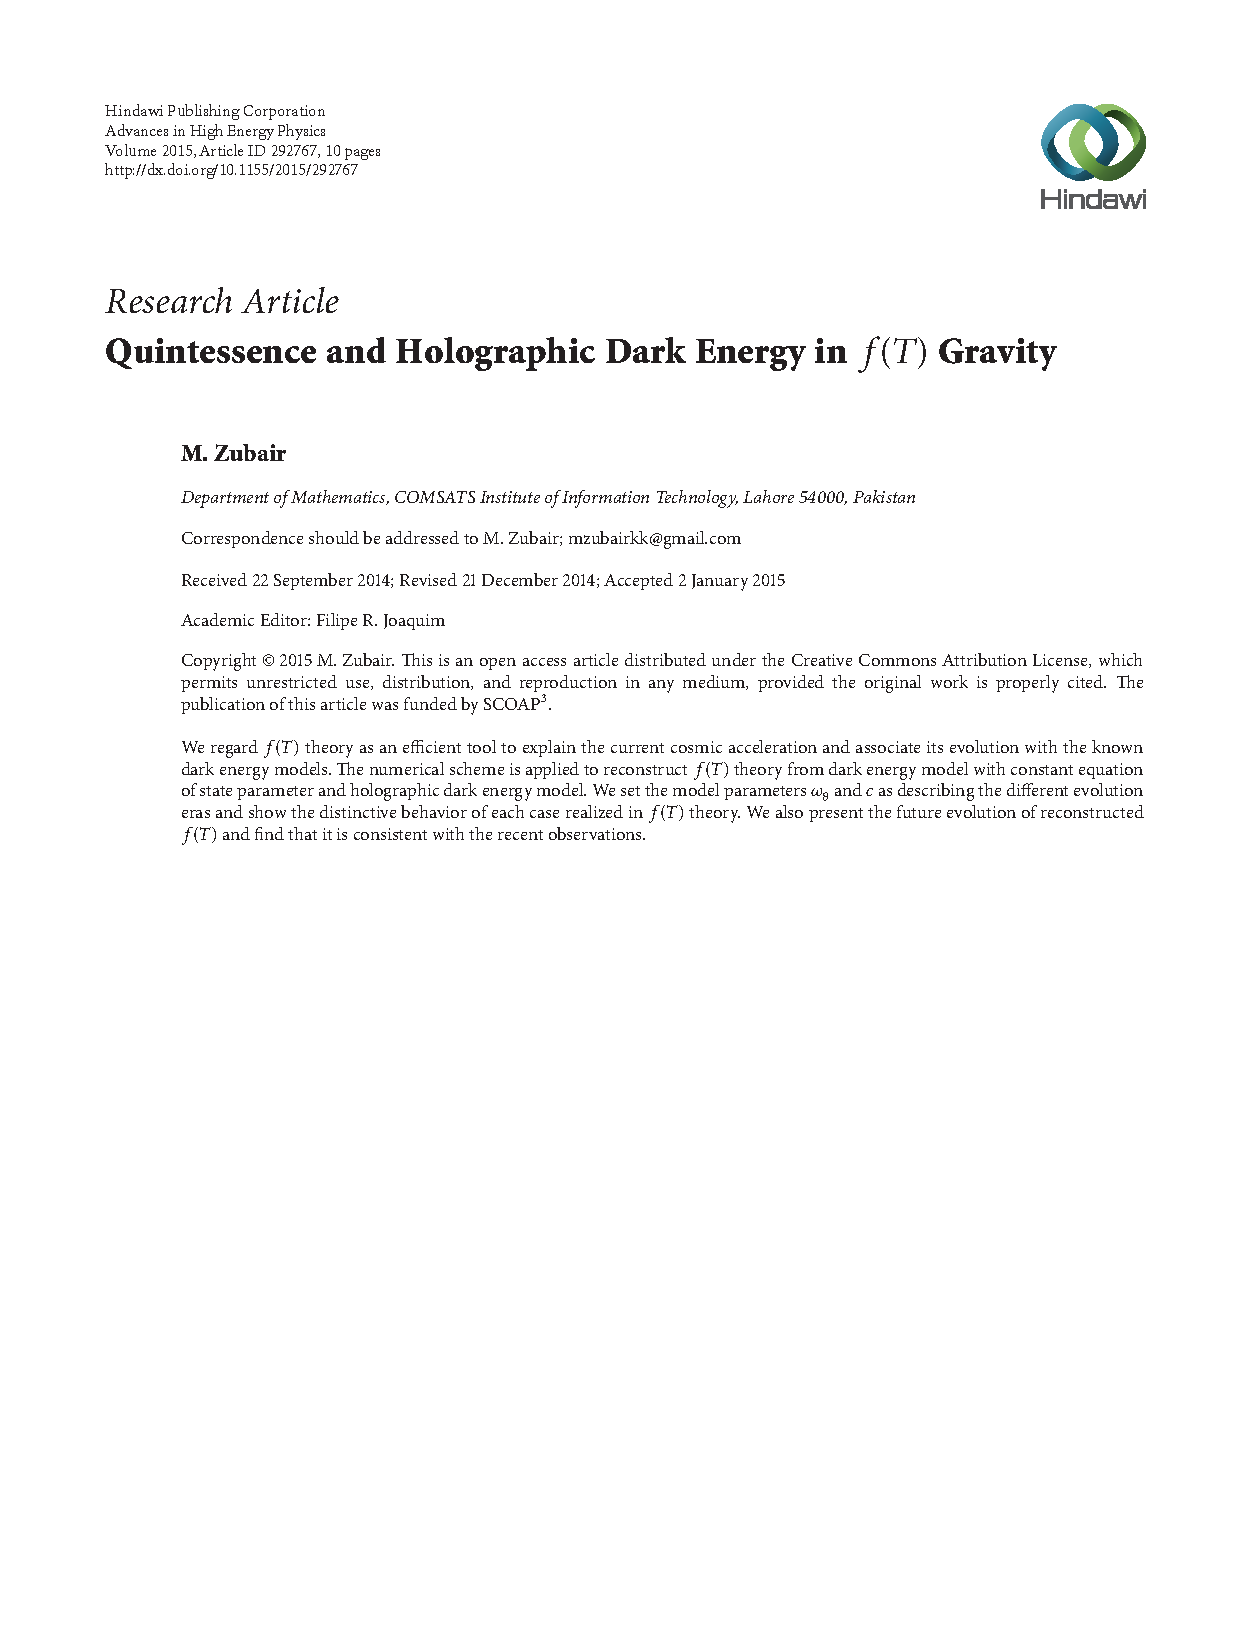
\includegraphics[width=3.25in]{Figures/header2.pdf}
\caption{The header section of a HEP paper.}
\label{fig:HMM}
\end{figure}

%% Appendix C

\chapter{Statistical Tests} % Main appendix title

\label{AppendixC} % For referencing this appendix elsewhere, use \ref{AppendixA}

\lhead{Appendix C. \emph{Statistical Tests}} % This is for the header on each page - perhaps a shortened title

To substantiate our claim that stop word frequency varies according to header section, we computed the frequency of stops words in  abstract, author list, and title sections for 20 HEP papers (\texttt{anova\_data.py}). Plotting these frequencies (Figure \ref{fig:means}) showed a drastic difference

\begin{figure}[!ht]
\center
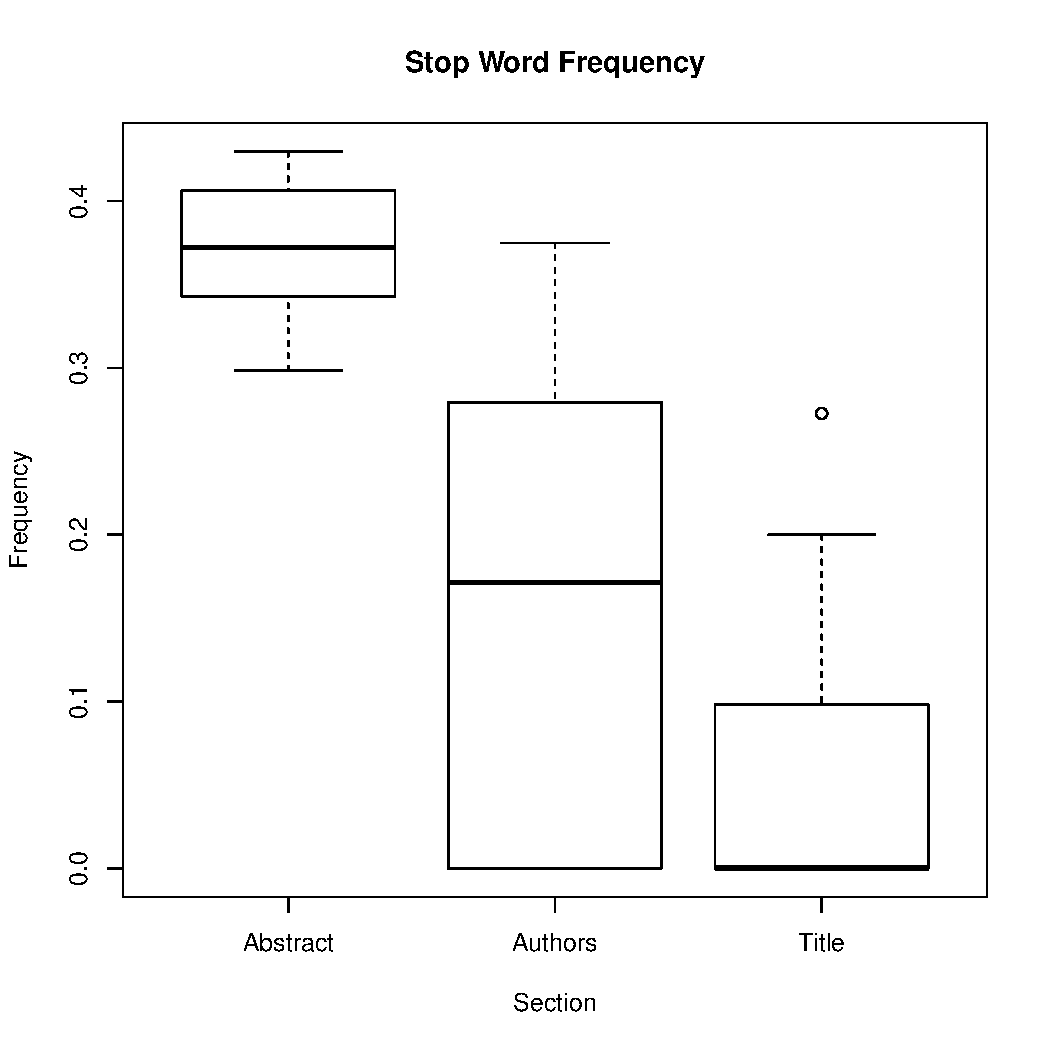
\includegraphics[width=4.5in]{Figures/means.pdf}
\caption{Box plots of stop word frequency according to header section.}
\label{fig:means}
\end{figure}

To confirm the significance of this result, we first performed an ANOVA (Figure \ref{fig:anova}) on the frequency data. The test reported a p-value of ($< 0.01$), permitting us to reject the null hypothesis that the means are equal ($\text{H}_0: \mu_1 = \mu_2 = \dots = \mu_k$), thereby confirming the statistical significance of the varying means. We further performed pairwise t tests (Figure \ref{fig:ttest}) to show the significance of the result for each class, with each p-value of ($< 0.01$).

\begin{figure}
\centering
\begin{BVerbatim}
            Df Sum Sq Mean Sq F value  Pr(>F)
Section      2 1.0685  0.5342   57.28 2.3e-14 ***
Residuals   57 0.5317  0.0093                    
---
Signif. codes:  0 ‘***’ 0.001 ‘**’ 0.01 ‘*’ 0.05 ‘.’ 0.1 ‘ ’ 1
\end{BVerbatim}
\caption{Excerpt of capitalisation features templates or \emph{macros}.}
\label{fig:anova}
\end{figure}

\begin{figure}
\centering
\begin{BVerbatim}
	Pairwise comparisons using t tests with pooled SD

data:  stops and sections

        Abstract Authors
Authors 1.5e-08  -      
Title   1.6e-14  0.0016

P value adjustment method: bonferroni
\end{BVerbatim}
\caption{Excerpt of capitalisation features templates or \emph{macros}.}
\label{fig:ttest}
\end{figure}


\addtocontents{toc}{\vspace{2em}} % Add a gap in the Contents, for aesthetics

\backmatter

%----------------------------------------------------------------------------------------
%	BIBLIOGRAPHY
%----------------------------------------------------------------------------------------

\label{Bibliography}

\lhead{\emph{Bibliography}} % Change the page header to say "Bibliography"

\bibliographystyle{unsrtnat} % Use the "unsrtnat" BibTeX style for formatting the Bibliography

\bibliography{Bibliography} % The references (bibliography) information are stored in the file named "Bibliography.bib"

\end{document}  